%% ----------------------------------------------------------------
%% Thesis.tex -- MAIN FILE (the one that you compile with LaTeX)
%% ----------------------------------------------------------------  


% Set up the document
\documentclass[a4paper, 11pt, oneside]{Thesis}  % Use the "Thesis" style, based on the ECS Thesis style by Steve Gunn
\newcommand{\setimp}{\newif \ifimp \imptrue}
\newcommand{\unsetimp}{\newif \ifimp \impfalse}

% change the below line to \setimp to switch to implementation phase template
\setimp

% Include any extra LaTeX packages required
\usepackage[square, numbers, comma, sort&compress]{natbib}  % Use the "Natbib" style for the references in the Bibliography
\usepackage[nottoc]{tocbibind} % bind bibliography to the table of contents
\usepackage{verbatim}  % Needed for the "comment" environment to make LaTeX comments
\usepackage{vector}  % Allows "\bvec{}" and "\buvec{}" for "blackboard" style bold vectors in maths
\usepackage[table]{xcolor}
\hypersetup{urlcolor=black, colorlinks=true}  % Colours hyperlinks in black, can be distracting if there are many links and colored blue.
\usepackage{graphicx}
\graphicspath{{Figures/}}  % Location of the graphics files (set up for graphics to be in PDF format)

%% ----------------------------------------------------------------
\begin{document}
\frontmatter      % Begin Roman style (i, ii, iii, iv...) page numbering

% Set up the Title Page
\title  {Drowsiness Detection System}
\authors  {Sheariff moustafa}
            
\addresses  {\groupname\\\deptname\\\univname}  % Do not change this here, instead these must be set in the "Thesis.cls" file, please look through it instead
\date       {\today}
\subject    {}
\keywords   {}

\maketitle
%%   ----------------------------------------------------------------

\setstretch{1.3}  % It is better to have smaller font and larger line spacing than the other way round

% Define the page headers using the FancyHdr package and set up for one-sided printing
\fancyhead{}  % Clears all page headers and footers
\rhead{\thepage}  % Sets the right side header to show the page number
\lhead{}  % Clears the left side page header

\pagestyle{fancy}  % Finally, use the "fancy" page style to implement the FancyHdr headers

%% ----------------------------------------------------------------
% Declaration Page required for the Thesis
\Declaration{

\addtocontents{toc}{\vspace{1em}}  % Add a gap in the Contents, for aesthetics

I, Sheariff moustafa, declare that this thesis titled, `Drowsiness detection System' and the work presented in it are my own. I confirm that:

\begin{itemize} 
\item[\tiny{$\blacksquare$}] This work was done wholly or mainly while in candidature for an undergraduate degree at Cork Institute of Technology.
 
\item[\tiny{$\blacksquare$}] Where any part of this thesis has previously been submitted for a degree or any other qualification at Cork Institute of Technology or any other institution, this has been clearly stated.
 
\item[\tiny{$\blacksquare$}] Where I have consulted the published work of others, this is always clearly attributed.
 
\item[\tiny{$\blacksquare$}] Where I have quoted from the work of others, the source is always given. With the exception of such quotations, this project report is entirely my own work.
 
\item[\tiny{$\blacksquare$}] I have acknowledged all main sources of help.
 
\item[\tiny{$\blacksquare$}] Where the thesis is based on work done by myself jointly with others, I have made clear exactly what was done by others and what I have contributed myself.
\\
\end{itemize}
 
 
Signed:\\
\rule[1em]{25em}{0.5pt}  % This prints a line for the signature
 
Date:\\
\rule[1em]{25em}{0.5pt}  % This prints a line to write the date
}
\clearpage  % Declaration ended, now start a new page

%% ----------------------------------------------------------------

% The Abstract Page
\addtotoc{Abstract}  % Add the "Abstract" page entry to the Contents
\abstract{
\addtocontents{toc}{\vspace{1em}}  % Add a gap in the Contents, for aesthetics
 This projects objective is being able to track a persons eyes or facial expressions for cues that would lead to the detection of drowsiness. The Drowsiness detection system will use eye tracking technology that is open sourced and computer vision libraries and tool kits such as openCV to develop a functioning Drowsy detection system,  Machine learning algorithms will also be used to successfully identify when a person is starting to fall asleep or the persons eyes are starting to close, Perclos is an algorithm used to detect if a persons is drowsy using the persons eyelid shape, once the system has detected that the persons eyes have been closed it then emit a warning single to the driver by way of a loud sound that will wake the driver up prevent him from falling asleep.  

}

\clearpage  % Abstract ended, start a new page
%% ----------------------------------------------------------------

\setstretch{1.3}  % Reset the line-spacing to 1.3 for body text (if it has changed)

% The Acknowledgements page, for thanking everyone
\acknowledgements{
\addtocontents{toc}{\vspace{1em}}  % Add a gap in the Contents, for aesthetics

I want to Kindly thank my Family for supporting me through out my time in collage and for my supervisor John Creagh for offering support through out the semester by offering help when needed and giving guidance and support. I am deeply appreciative and grateful for all the support and hard work.   \ldots

}
\clearpage  % End of the Acknowledgements
%% ----------------------------------------------------------------

\pagestyle{fancy}  %The page style headers have been "empty" all this time, now use the "fancy" headers as defined before to bring them back


%% ----------------------------------------------------------------
\lhead{\emph{Contents}}  % Set the left side page header to "Contents"
\tableofcontents  % Write out the Table of Contents

%% ----------------------------------------------------------------
\lhead{\emph{List of Figures}}  % Set the left side page header to "List if Figures"
\listoffigures  % Write out the List of Figures

%% ----------------------------------------------------------------
\lhead{\emph{List of Tables}}  % Set the left side page header to "List of Tables"
\listoftables  % Write out the List of Tables

%% ----------------------------------------------------------------
\setstretch{1.5}  % Set the line spacing to 1.5, this makes the following tables easier to read
\clearpage  % Start a new page
\lhead{\emph{Abbreviations}}  % Set the left side page header to "Abbreviations"
\listofsymbols{ll}  % Include a list of Abbreviations (a table of two columns)
{
% \textbf{Acronym} & \textbf{W}hat (it) \textbf{S}tands \textbf{F}or \\
\textbf{LAH} & \textbf{L}ist \textbf{A}bbreviations \textbf{H}ere \\

}

%% ----------------------------------------------------------------
% End of the pre-able, contents and lists of things
% Begin the Dedication page

\setstretch{1.3}  % Return the line spacing back to 1.3

\pagestyle{empty}  % Page style needs to be empty for this page
\dedicatory{For/Dedicated to/To my\ldots}

\addtocontents{toc}{\vspace{2em}}  % Add a gap in the Contents, for aesthetics

%% ----------------------------------------------------------------
\mainmatter	  % Begin normal, numeric (1,2,3...) page numbering
\pagestyle{fancy}  % Return the page headers back to the "fancy" style

\chapter{Introduction}
\label{chap:intro}
\lhead{\emph{Introduction}}\textbf{}

For my final year project I have tasked myself with developing a drowsiness detection system, with the objective of being able to track a persons eyes or facial expressions for cues that would lead to the detection of drowsiness. The Drowsiness detection system will use eye tracking technology which may be open sourced or developed using certain programming  library's to successfully identify when a person is starting to fall asleep or the persons eyes are starting to close, once the system has detected that the persons eyes have been closed it then emit a warning single to the driver by way of a loud sound that will wake the driver up prevent him from falling asleep.  


\section{Motivation}
Drowsiness occurs when a individual person starts feeling sleepy, its a feeling of sleepiness and is one of leading causes behind vehicle crashes by motorist all over the world. The Road Safety Authority is the leading body responsible keeping the roads safe in Ireland, they try to make roads safer by reducing the number of injuries and the severity of these injuries. 

The road safety authority have stated that the " Drivers suffering from a sleep debt are at risk of ‘nodding off’ whilst driving and substantially increasing their risk of being involved in a crash. It is estimated that driver fatigue is a contributory factor in as many as 1 in 5 driver deaths in Ireland every year. Furthermore, tiredness-related collisions are 3 times more likely to be fatal or result in a serious injury because of the high impact speed and lack of avoiding action. A survey* of drivers’ attitudes to driver fatigue conducted by the Road Safety Authority in 2014 revealed that over 1 in 10 motorists have fallen asleep at the wheel.  The survey also found that motorists who drive as part of their work, and motorists who admit to driving after taking any amount of alcohol, had a higher than average incidence of falling asleep at the wheel (almost 1 in 5 fell asleep at the wheel)". 
Also ( "A study by the AAA Foundation for Traffic Safety estimated that 328,000 drowsy driving crashes occur annually. That's more than three times the police-reported number. The same study found that 109,000 of those drowsy driving crashes resulted in an injury and about 6,400 were fatal"). 

When looking at these local and global figures I always wondered if there was a way to reduce these numbers with the hope of saving lives, lower the amount of crashes and reduce damages to the driver, environment and to the insurance companies that have to pay out money for damages that may have happened to another persons vehicle or property. I do feel these accidents can be avoided with some ingenuity, this has lead me to research and to develop a drowsiness detection system in order to detect drowsiness behind the wheel, also I do wish to develop the drowsiness detection system as a solution for other environments, for example jobs which require people to work at higher altitudes or under higher G-Force such as jobs that require jet flight. These types of jobs are dangerous due to the lower oxygen levels that go along with the tasks that are associated while performing these jobs and due to the decreased concentration levels of oxygen in the air this can result in the person losing consciousness because the human body needs a certain level oxygen within per to be available in there blood and more specifically a good level of oxygen must be received by there persons brain or else the brain will not be able to perform effectively, so I do believe that my motivation with this project is that I can tackle a common local and global problem and also a problem that occurs to humans naturally due to environment that person is in.
\section{Contribution}
During my time in collage I have  taken many modules that aided me towards  the completion of this project such as Linear data structures and algorithms, this module helped me develop better technical programming skills such as being able to use recursion to help aid me when i am developing my projects, this didn't just improve my coding skills it helped me develop a stronger coding sense. object orientated principles/ object orientated programming module,  both of these modules have taught me the fundamentals of programming in java which have helped me to easily understand other programming languages such as C and Python very easily as the logic used in these languages is very similar to java not only by learning these language, undertaking both of these modules have allowed me understand things such as inheritance, serialization, super classes and the ability to develop GUI's and techniques to help send information to a back end database such as MY-SQL. Programming Data analytic was another excellent module that is crucial to the completion of my Drowsiness detection system as python was taught in this module and this is the core programming language used to develop my project. python is Versatile, Easy to Use and Fast to Develop with, contains many libraries and technologies that helped me develop my Drowsiness detection system. Distributed system programming aided me by teaching me how to communicate between two different application (Server and client)  to fulfill tasks by sending information between them along with multi-threading/synchronization by the means of messages. 

\section{Structure of This Document}
When looking through this document You will notice that most of the work done in this Document will be the chapters 2 and 4 while the remaining chapter 1  chapter 3 and chapters 5 consists of work done by myself, but does not have as much work as the other chapters.
\subsection{Chapter 2}
In chapter 2  The chapter starts off with how the drowsiness detection system places itself within the thematic area in computer science this section consists of how This system positions itself within computer science. The chapter then goes on to detail all the research paper, blogs and websites that have been read and cited followed by the state of the art which is what is being done with the drowsiness detection system today actively.
\subsection{Chapter 3}
This chapter is far more brief and the issue tackled in this chapter is the problem that the drowsiness detection system will tackles the requirements that it must achieve, the functional and non functional requirements and the objective that the systems  must achieve.
\subsection{Chapter 4}
This chapter is basically a detail of how the drowsiness detection system will be designed and implemented going forward with the implementation of the system. The chapter is broken up into  headings such as architecture which has subheadings consisting of design models, technologies, databases and frameworks of the drowsiness detection system. followed by another heading called risks. Within risks there is a detail of all the risks that this system could encounter while going forward with the implementation. Other headings called methodologies and implementation plan schedule will follow shortly as separate heading. In the methodology heading their is discussion on what agile philosophical methods will be used to delegate work in semester 2, while the implementation plan schedule will consist of tasks that I have outlined and will achieve for semester 2, after this there is another 2 separate headings evaluation and prototype. For the evaluation portion you will just find a short summary of how I will analyse the projects success and how i will accept things in this System to be a success during the implementation phase. The prototype heading will consist of a short test of the technologies that my system will be using during the second semester.
\subsection{Chapter 5}
This is a very short chapter and consist mostly of a reflective opinion of the work done on this document as-well as things that i have achieved and didn't. This chapter will consist of a overview,discussion, conclusion and future work. All of these are headings with brief reflections on my journey on work on this project. 




 % Introduction
\chapter{Background}
\label{chap:background}
\lhead{\emph{Background}}


Previous research on drowsiness detection was focused primarily on the lane deviation but due to to how late this detection was carried out the focus was changed to a more moderate solution that would try to detect the drowsiness of an individual well before an accident would occur, now that technology has advanced researchers are able to identify when a driver behind the wheel has become drowsy as the advancement in technology has allowed for precise detection of the symptoms that are exhibited when an individual behind the wheel starts to feel drowsy such as the bopping of the head, heart rate slowing down their eyes starting to feel heavy.

The leading cause of work related fatalities are driving related jobs. This is a big issue that corporations and road safety campaigners are trying to solve, due to the improvement in technology that we have access too we are able to develop technologies that can very accurately detect the symptoms associated with drowsiness.

Today we live in a world that is dictated by technology, this has resulted in tasks becoming much easier to accomplish - such as the ability to communicate with other people around the world, more information gets passed around much quicker. Applications have been on the rise since the introduction of the smartphone and so has fast food application. These application have resulted in a increase of fast food drivers especially in countries such as china who have seen a boom in food delivery couriers delivering food by scooters there has also been a increase in road accidents due to this. 

 
\section{Thematic Area within Computer Science}

The concrete topic that will be looked at here is how Drowsiness behind the wheel can be detected in a manner that is effective and reliable in the hope to increase the safety of drivers and workers behind the wheel who have been driving 
while also feeling sleepy, the aim is to detect when they have started to feel sleepy and to signal them to wake up. This is accomplished through eye tracking technology that would find behavioral signs that the driver may be exhibiting that are related to the drowsy driver, Making this a system that is very reliable is the main goal of the project. Using a small camera  the cost of this system will be minimized but cost effective for the user who uses the technology in their car. The camera can be placed in front of the driver just above him so that it doesn't obstruct his field of view while he is driving also maintaining the reliability that the camera will work effectively in catching drowsiness as they are driving their vehicle
  
The core Area this project falls under within computer science is as a embedded application. The software is the core of this system as it will run the functionality needed for the camera to perform the tasks needed by the user. The software will carry out all the operations such as  the driver while the camera while be responsible with detecting the driver when he starts feeling sleepy behind the wheel.

The main area this project falls under is embedded engineering.
\textbf{
\section{Project scope}
}
\textbf{Embedded applications}

Embedded applications are software applications that permanently reside within a device, providing some type of control function or user interface. The software is currently stored within the read only memory (ROM) or within flash memory. The reason why software get stored in the ROM is because if for any chance the power supply to the device is stopped for whatever reason then the application that is embedded within the device will not get erased and will still be available to run the functionality that was intended, so to makes things simple ROM stores the program code while the random access memory (RAM) stores the transient input and output data. Embedded applications are in nearly every piece of hardware that we use and can be very complicated or very simple depending on the function that the hardware has to carry out, some small embedded applications such as the ones inside a microwave don't require a operating system to control them, other more complex systems such as entertainment systems that are in control of a multitude of channels and are expected to record and play videos from a large and wide range of devices will need an operating system to manage the resources in real time. Real time Embedded systems are thing such as a GPS navigating system (Global Positioning System), industrial robots, traffic monitoring system, smart phones and smart TV's all of these embedded system all have applications dictating the functionality of these devices.

Embedded versions of popular operating systems like Linux, Windows and Mac are available, along with some specialized OSes. They will usually have reduced storage needs and will work with less RAM than a desktop OS. The program instructions for embedded systems are called firmware, or embedded software. Embedded software is typically very easy on hardware resources – requiring little memory and often needing no keyboard or screen. The embedded software is not controlled by human interfaces, but rather by machine interfaces.
In this project a small  camera will be used, any computer has a built in front facing camera and this will be the hardware used to analyse the eye closure rate of the driver. This will be the embedded hardware used in the project. The camera will constantly take images so that it can compare the images with previous images that are stored in a database.    

\textbf{Background operations}
In the background there will be an application running that will track the eye movement of the driver. Thanks to readily available open sourced eye tracking software and libraries that is easily available to download from the internet, we have access to useful tools that are will work in conjunction with the camera to detect drowsiness. The use of the Python language adds another advantage in the fact that its the most used language in the world this has resulted in a wide range of libraries and technologies that can works with this programming language.  Using Python to communicate with embedded systems
Python scripts can put the system into different states, set configurations, and test all sorts of real-world use cases. Python can also be used to receive embedded system data that can be stored for analysis this is essential within the project as the project has a huge analytical importance that will determine the applications success, using a programming language that fits well within the boundaries of the projects goals will be essential in achieving the unique goals and tasks that this project requires. 

\textbf{PyGaze and OpenCV}
The Python Supports many open source eye tracking technologies, PyGaze is a open sourced toolbox for eye tracking in python it also has two accompanying features  PyGaze analyser and webcam eye-tracker, PyGaze will be useful in analyzing the users eye movement such as the what the user is looking at within that particular moment if he is fixated on something or is shifting his gaze elsewhere. Using the information that is gathered from the the open source software we can then trigger the event detection methods that are within the python script to help use form a conclusion. The methods within PyGaze will be the main method used to gather information about the user, such as the direction of there gaze and eye lid distance for determining events such as if the user has stopped looking at the road and his gaze has gone downwards accompanied by his eyes shutting signally sleepiness.the benefit that this open source technology brings is that it is very accurate as it has been tried and tested. 

OpenCV is an open source computer vision and machine learning software library. OpenCV was built to provide a common infrastructure for computer vision applications and to accelerate the use of machine perception in the commercial products.The library has more than 2500 optimized algorithms, which includes a comprehensive set of both classic and state-of-the-art computer vision and machine learning algorithms. These algorithms can be used to detect and recognize faces, identify objects, classify human actions in videos, track camera movements, track moving objects, extract 3D models of objects, produce 3D point clouds from stereo cameras, stitch images together to produce a high resolution image of an entire scene, find similar images from an image database, remove red eyes from images taken using flash, follow eye movements, recognize scenery and establish markers to overlay it with augmented reality. OpenCV will be used in conjunction with PyGaze, it will analyse the data received by the PyGaze and run it through set algorithms in order to detect any abnormalities that may be occurring to the user my be exhibition that may lead to a successful and accurate detection.

\textbf{Machine Learning Techniques}
Machine learning techniques and algorithms must be used in this project in order to fulfill the tasks that are required of this projects, these techniques may range from the Haar cascade classifier algorithm to multiple other automatic classifier algorithms. These algorithms will be primarily pattern algorithms that will help the camera detect drowsiness, the cascade classifiers are excellent algorithms and are perfect for this type of project because the cascade function is trained from a lot of positive and negative images. It is then used to detect objects in other images. Initially, the algorithm needs a lot of positive images (images of faces) and negative images (images without faces) to train the classifier. Then we need to extract features from it, this is tedious but an effective method to detect facial features such as eyes. The core of these techniques imply use probability factors to determine whether an alert should be raised.  These problems are  classified  between  classification,  regression,  clustering  and  distribution. This project will mainly deal with classification based machine learning algorithms some regression based algorithms may be used to determine if the user is drowsy from the data. They are built up over time using time-series analysis, where the algorithm adapts and evolves as new information is fed to it. The images that are fed to the cascade classifier must be taught slowly on how to detect eyes by slowly introducing new features to the algorithm from faces to eyes, we do this by slowly introducing new areas of the face. The machine learns to detect new faces by using a positive value for images with a face and a negative value for images without a face, eventually the machine will be able able to detect certain features after gradually working the algorithm to the target feature that is desired. In the case of this project the target feature will be the eyes.

\textbf{Human computer interaction}
Human-computer interaction (HCI) is a multidisciplinary field of study focusing on the design of computer technology and, in particular, the interaction between humans (the users) and computers. While initially concerned with computers, HCI has since expanded to cover almost all forms of information technology design. The interaction that the user will have with the camera is important because it must be in a manner will allow the camera to successfully gain the data from the user and for the user to benefit from the camera in a way of preventing him from falling asleep. This interaction is essential for this project to be successful in achieving its goals. This is the essence of HCI, having the best form of interaction between the embedded device and the user will help achieve the users needs

\section{A Review of -INSERT THEMATIC AREA-}

  \textbf{Eye Tracking technology to detect drowsiness}
               
Eye Tracking System to track Driver drowsiness by Nguyen, T.P. and Chew, Moi Tin and Demidenko, S.N. \cite{article} This study focuses on analysing the available algorithms and the techniques so that eye detection rate can be as accurate as possible The conclusion was that a viola Jones and Perclos method both achieved the highest eye detection rate. 

Real Time Eye Tracking and Detection-A Driving    Assistance System by Said, Sherif and Beyrouthy, Taha and Hassan, Murtaza and Fayek, M and Al Kork, Samer, \cite{reference2} This study focuses on a driver attention while behind the wheel using eye tracking technology and a wearable bracelet, a in-vehicle  information systems is also used to monitor when the driver gets distracted behind the wheel.

Drowsiness Detection System for Pilots by Muniyandi, Manivannan and Singh, Gurpreet    \cite{inbook} This study discusses primarily on how to detect when an individual is showing signs of sleep-onset while using non intrusive methods. The study uses individuals pupil diameter while keeping a threshold deviation of +5 for both pupils. The scope of the paper was to evaluate algorithm which  was  used to  separate out  the  events which  are encountered  while  monitoring  the  eye pupil  of a  subject.  

Real-time monitoring of driver drowsiness on mobile platforms using 3D neural networks by Jasper S. Wijnands, Jason Thompson, Kerry A. Nice, Gideon D. P. A. Aschwanden, Mark Stevenson \cite{study} This study discusses the possibility of bringing a drowsy detection system to mobile phones by application using a 3D neural network, It discuses how the application was built and the issues it tackled developing the application to provide an accurate system.


\textbf{wearable devices }
 Electrodermal Activity Based Wearable Device for Drowsy Drivers by Malathi, D and Jayaseeli, Dorathi and Madhuri, S and  Senthilkumar, K.     \cite{article2 } This article looks at monitoring the skin using a wearable device in order to evaluate if a individual is is starting to feel drowsy due to the sweat levels that the body is releasing. The main goal of of this study it to determine the mental state of a driver at a given time by monitoring the brains subconscious activities such as sweat being released from the sweat glands in the skin.
 

\textbf{ Journals}
Smart Real-Time Video Surveillance Platform for Drowsiness Detection Based on Eyelid Closure by Muhammad Tayab Khan,1 Hafeez Anwar,2 Farman Ullah,2 Ata Ur Rehman,2 Rehmat Ullah,3 Asif Iqbal,4 Bok-Hee Lee,5 and Kyung Sup Kwak4\cite{journal} This article sets out by trying to establish drowsiness detection by using the drivers eyelids and the curvature of the eyelids using sobel operators and also the viola-jones algorithms. 

\textbf{Blogs}
Real time Driver Drowsiness Detection (Sleep Detection) by Taha Emara\cite{blog1} This blog discusses Dlib, a c++ toolkit and can be used for python projects also. This blog discusses how this toolkit is excellent for Drowsiness detection as it provides landmarks points that outline the eyes and face, each eye has 12 points and these point are used to compute the eye aspect ratio to estimate the level of eye opening.

DROWSY DRIVER DETECTION SYSTEM: A NEW SAFETY FEATURE by MATTHEW C. KEEGAN\cite{blog2} This blog briefly discusses the issue of micro sleep on the road which lasts between a single milliseconds and 15 seconds and its dangers, also discusses the the work companies are doing to develop detection systems and the methods these systems are implementing, as well as discussing how in the future cars will be able to take over when the system within it detects drowsiness .

Panasonic Reveals Drowsiness Detection System to Combat Driver Fatigue by PRWK\cite{blog3} This blog discusses how Panasonic Bosch and Plessey Semiconductors will be releasing Drowsiness detection technology Panasonic will be using an in-vehicle camera to recognize, analyze, and measure the rate of a driver’s blinking eyes and changes in facial expressions that may indicate fatigue, Bosch will develop a camera system similar to Panasonic’s that monitors a driver’s head and eye movements, posture, and body temperature to measure fatigue while Plessey Semiconductors  has developed seat sensors to monitor heart rate change, using an algorithm to monitor breathing changes consistent with fatigue to provide the driver with advanced warning before potentially feeling the effects of fatigue

\textbf{
\section{Current state of the art}
}
This segment of the paper surveys and examines the most recent advancements in connection to drowsy detection in order to decide how best to take care of the problem at hand. Luckily, an incredible amount of work has  been done  on this topic and this area looks at a wide scope of these works, including works from the above segments There is a huge amount of methods  by which drowsiness detection has been actualized so we analyze these in detail. We mean to reveal the latest improvements in the field that will take care of our concern, and talk about how different works can be based upon to actualize an answer for the current issue. Before the finish of this segment we ought to have a reasonable comprehension of what has been engaged with drowsy detection. This area is isolated into a few sub segments which portray various orders or current patterns inside the field of drowsy detection.
\textbf{
\subsection{Detection methods}
}
Currently when it comes to drowsy detection systems and to having an effective drowsy detection system there is 2 different paths that other individuals who have tried to tackle this problem have taken and that is either going by an non intrusive method such as image and video processing or a more intrusive method such as wearable like wristbands which can detect a persons sweat levels that is being released, these are methods used to analyse the brain of the individual to catch subconscious triggers that can lead to accurate detection of sleepiness, our solution will be through non intrusive means so naturally we will have to look at eye technology as a solution to this problem.
current modern techniques that are used today to solve this issue is by using eye tracking technology, the issue is finding the best techniques with this technology to have a successful system, techniques that are currently used are  eye closure
ratio, eye blinking, head position, facial expressions, and yawning. Eye tracking technology is now advanced enough to detect even the smallest deviations in the pupils of an persons eyes from a distance of 2 meters. PERCLOS method is the most frequent used metric when it comes to drowsy detection based on eye state observation at the moment. PERCLOS is the ratio of eye closure over a period and from this being able to determine if an eye is open or closed. My solution to this problem will mainly use the users eyes as a solution this projects problem. 
PERCLOS =No. frames of closed eyes/3 min interval of all frame blinking time
Yawning based detection systems are also used to detect Drowsiness and can be a very accurate method for this solution. yawning based detection systems analyse the variations of the geometric shape of the drowsy persons mouth and lip position, wider opening of the mouth on a regular basis is usually a dead give away when it comes to detection by this method.
Behavioral based techniques are used also to achieve this computer vision and a Camera is usually used to capture behavioral actions that the a person may exhibit. The current issues when using this method are usual environmental factors, such as the illumination, brightness,and road conditions influence the credibility and accuracy of measurement and this makes it very unreliable when trying to have an accurate system. \cite{ramzan2019survey}, we will delve deeper into these detection methods and see in detail how these solutions work currently.

\textbf{ EYE TRACKING AND DYNAMIC TEMPLATE MATCHING}
 When trying to avoid road accidents, a real time driver fatigue system based on vision is proposed to tackle this problem \cite{ramzan2019survey}. This solution is currently the most used solution that other individuals have tried to use to solve this issue, usually the system detects  the face of the driver from the input images using HSI (hue , saturation, intensity)color model which  decouples the intensity component from the color-carrying information(hue and saturation) in a color image. The HSI model is an ideal tool for developing image processing algorithms based on color descriptions that are natural and intuitive to humans, it then uses the sobel edge operator which sometimes called the Sobel–Feldman operator or Sobel filter, is used in image processing and computer vision, particularly within edge detection algorithms where it creates an image emphasising edges \cite{ramzan2019survey}.  The Sobel edge operator is used to locate the eyes positions and gets the images of eye as the dynamic template for the tracking of eye. Then the obtained images are converted to HSI color model to decide that whether the eyes are close or open to judge the drowsiness of driver

\textbf{MOUTH AND YAWNING ANALYSIS}
Fatigue is one of the main reasons that road accident do occur to avoid this issue one of the main solutions is using facial images to detect drowsiness \cite{saradadevi2008driver} Firstly, the system locates and tracks the mouth of a driver using cascade of classifier training and mouth detection from the input images. A Haar Cascade is basically a classifier which is used to detect the object for which it has been trained for, from the source. The Haar Cascade \cite{inproceedings} is trained by superimposing the positive image over a set of negative images. The training is generally done on a server and on various stages. Then, the images of mouth and yawning are trained using SVM.  An SVM model is a representation of the examples as points in space, mapped so that the examples of the separate categories are divided by a clear gap that is as wide as possible. New examples are then mapped into that same space and predicted to belong to a category based on the side of the gap on which they fall.
SVM is used to classify the regions of mouth to detects the yawning and alerts for fatigue.\cite{yeo2009can}

\textbf{FACIAL EXPRESSIONS METHOD}
 Finite Element Analysis is used by the researchers which is a complex system that contains the database of facial expression as a template and detect the drowsiness on the basis of results from database\cite{ramzan2019survey}. The proposed solution with this type of method is to have the hardware system use in fared d light as it has giving many benefits like ease of use, independent of lightning conditions of environment. The system firstly uses the technique of background subtraction to determines the face region from the input images. Background subtraction (BS) is a common and widely used technique for generating a foreground mask (namely, a binary image containing the pixels belonging to moving objects in the scene) by using static cameras \cite{wilkinson2013accuracy}. Then using horizontal projection and template matching, facial expressions are obtained. After that in the tracking phase, elements found earlier are followed up using template matching and then investigates the incidence of sleepiness using the determination of facial states from the changes of the facial components. Changing in the three
main elements such as eye brow rising, yawning and eye closure for the certain period are taken as the initial indications for drowsiness and the system generates the alert. The facial expression method does use a combination of the other methods to achieve its task but its a more accurate method as it detects multiple types of drowsiness.\cite{ramzan2019survey} 

\textbf{EYE CLOSURE AND HEAD POSTURES METHOD} 
 At first a  video is captured using webcam and for each frame of video the following operations are performed in order to detect the face and eyes, viola-jones method is then used. The Viola-Jones algorithm is a widely used mechanism for object detection. The main property of this algorithm is that training is slow, but detection is fast. after this the face is partitioned in to three areas and the top one presenting the eye area is browsed by the Haar classifier.\cite{ramzan2019survey} if Then to detect the eye state, Wavelet Network based on neural network is used to train the images then the coefficients learning images is compared with the coefficients of the testing images and tells which class it belongs. When the closed eye is identified in the frames then the eye closure duration is calculated using PERCLOS, if the value exceeds the predefined time then the drowsiness state is detected. Then the developed system estimates the head movements which are: left, right, forward, backward inclination and left or right rotation. The captured video is segmented into frames and extract the images of head and determines the coordinates of image. Then the images are compared to determine the inclined state of head and same case with other head postures.Finally, the system combines the eye closure duration and head posture estimation to measure the drowsiness. \cite{ramzan2019survey}

{
\subsection{Machine learning algorithms}
}
Solutions to drowsy detection systems have many Machine learning algorithms as these algorithms must be used to achieve the goal of this project, Different algorithms are used to achieve different task withing the context of this project. I will be discussing the most common algorithms that are used today with this project with he modern technology that is available to use.

\textbf{ cascade classifier}
This is a machine learning object detection algorithms used to identify objects in an image or video. Its an algorithm that is very popular within the context of my project and is used very often in facial analysis solution\cite{inproceedings}.The use of the cascade classifier algorithms help the camera recognise a face from a random object in the background.One of the algorithms that is most common with this project is the Haar cascade classifier algorithm. Once   the   Haar   features   are   obtained  then  individual  classifiers  are  built  based  on  the  values  of  each  Haar  feature.  These  individual  classifiers  are  then arranged into a cascade classifier. A cascaded classifier is combination  of  several  classifiers  arranged in different  stages to cascaded on after one another. The number of classifiers in each stage and their threshold values are determined by the boosting algorithm during the training of the classifiers with labeled face images. Boosting algorithms work well with this algorithm as if helps the algorithm improve facial detection. A boosting algorithm is  family of algorithms which converts weak learner to strong learners. \cite{inproceedings1}

\textbf{SVM}
Support Vector Machine is a supervised machine learning algorithm which can be used for both classification or regression challenges. However, it is mostly used in classification problems, this algorithm is very common in drowsy detection systems also and works in sync with the Haar cascade classifier. The SVM algorithm is used to train the cascade classier on the regions of the face the individual want to analyse to carry out the function of the  project. SVM is used to classify \cite{Source1}
the regions in the image that you want to focus on, such as the eyes mouth the regions of these areas such as the eye lids or mouth geometry that is being expressed in the image.If the result of the classification indicates that the driver’s eyes is closed for a predefined period of time, the eyes of the driver will be considered closed and hence an alarm will be started to alert the driver, or if the result of the classification indicates that the drivers lips are to far apart of that maybe the geometry is not normal for a  predefined period of time then the drivers lips may be considered open and the alarm will be started to alert the driver.

\textbf{PERCLOS}
This is an algorithm used in this project to measure eye closure and is very effective in achieving this.This method is very common within the fatigue detection system. PERCLOS is a drowsiness detection measure, referred to as the percentage of eyelid closure over the pupil over time and reflects slow eyelid closures or droops rather than blinks\cite{journal}, this algorithm has the highest accuracy when it comes to eye closure detection. This method is a staple when it comes to to detecting behavioral cues and one of these cues is the drowsy individuals eye closure rate.

\textbf{viola - Jones}
viola-Jones method is also very common and is used to partition images into sections, usually within the context of this project face gets partitioned into three areas and the top one presenting the eye area honed in on.The Viola–Jones object detection framework is the first object detection framework to provide competitive object detection rates in real-time. within the context of this project this method work by detecting the eyes in the frame in real time. when the closed eye is detected then When the closed eye is identified in the frames then the eye closure duration is calculated, if the value exceeds the
predefined time then the drowsiness state is detected.\cite{teyeb2014drowsy} Head posture doesn't matter as this algorithm is able to  take constant sample from the individual and test it with the previous images regardless of the posture that the user is expressing.



 % Background Theory 
\chapter{Drowsiness detection system}
\label{chap:problem}
\lhead{\emph{Problem Statement}}

\section{Problem Definition}

The objective of this project is to tackle a problem that is one of the core problems behind road accidents and has been tackled by many different individuals who have taken on this project with the aim of trying to solve the problem of drowsiness behind the wheel, but finding a single effective method to solve this problem has been very challenging as there has been a split on the method used to detect drowsiness for example should one use a  evasive method by monitoring the eyes lids of the drowsy individual using a camera or by using bracelet's and heart beat monitors as a more non evasive method for analysing drowsiness.The situation that arises at this point is to question which method will be the best in resolving and tackling this problem, what is the most effective in detecting if a driver is drowsy or not some studies have Incorporated both evasive and non evasive methods and some have decided to go with one or the other but for detecting of a driver is drowsy or not has to come down to the evasive method by using a camera to monitor the eyelids of the driver using the PERCLOS equation which takes a percentage of eyelid closure, the equation is calculated by counting the number of frames in which there was no pupil detected, and dividing this by the total number of frames for a specific time interval, PERCLOS  has a very high accuracy and is used  by continuously by others who have researched fatigue based projects its the leading evasive method.

Detection of events in this system is will be  instantaneous as the user is constantly being monitored by a camera which will return readings about the drivers state to a computer that will process the drivers state. Currently the methods  that  exist only alarms the drivers but doesn't give any other functionality such as a management system or by keeping a track record of the drivers behavioral history.  The system being proposed by this project wont only just alarm the driver it will keep track of how many drowsy detection have happened lately for the driver  and will have a management system that also monitors the driver and can notify the driver to take a rest if required, each drowsy alert the system detects management will receive a notification also which will increase the safety of the driver and reduce the number of fatal crashes on the road. 




\section{Objectives}
•Have a fully functioning detection system that has a management and back end database system in place .

•Accurately detect if a driver is feeling drowsy.

•Be able to notify the driver with an alarm if drowsiness has been detected.

•The application has to be evasive and not bother the driver.

•The application has to be easy to configure and calibrate .
\section{Functional Requirements}

\subsection{Application requirements}

•The camera used must run with a minimum of 5 megapixels.

•The alarm should have a minimal sound of 65 db(A)to 5 dB(A) in order to wake the driver  .

•Their must be a notification sent to the management after every alarm trigger.

•A message must be sent to the driver if the alarm has been triggered more then once within a short space of time .

•The alarm must be consistent until the driver becomes alert again .

•A prompt appears if the driver doesn't respond to the alarm within a specific time frame usually anything over 5 seconds

\subsection{Database requirements}

•The database must keep track of the drivers details

•If the driver has a history of drowsy driving the driver will be categorically placed in a high risk section on the database

•The database will have the vehicle details 

•A user view the history of the driver through the database

• A user can add and remove  drivers from the database

• Drowsiness information will be displayed for each user in a table and will be updated as received.

•Heart rate information is displayed for each user in a graph and it updates as new information is received.


\section{Non-Functional Requirements}

•The application must accommodate all camera sizes.

•The application must be able to sound any of alarm type.

•The camera must work under any light conditions

• The alarm will be heard under any conditions regardless

•Notification alert to be triggered through:
         –Multiple alarms going off within a short term basis .
         –Alarm going off due to sleepy driver.
         –Drowsiness detection by camera

• The drivers details will be set up on the database when the driver sets up the drowsy detection system for the first time .







 % Problem
\chapter{Implementation Approach}
\label{chap:implementation}
\lhead{\emph{Implementation Approach}}
\usepackage{graphicsx}

Identifying the best technologies to utilise in order to design the drowsiness detection system enables the objectives of the project to be met.  Understanding how each technology would fit into the architecture and function with one another meant researching various alternative approaches. In order for me to fully design and implement this project successfully I will need to carefully layout out a path to successfully build my project from the ground up while trying to minimize all the issues that I will encounter on the way.
Now I must specify my initial first understanding of what the system is required to do, I will look at drafting a first outline of a software system to meet the requirements that must be met in order of fulfilling the task of fully. It is not the goal of this outline to prescribe the implementation of every detail of the system, but rather to gain an overall idea of the technologies, subsystems and components involved; their relationship to each other; and the role they play in the system. It also presents us with another chance to uncover complex, badly understood, or other potentially problematic areas of the system—crucial knowledge when it comes to estimating the work load (cost) during the planning of the project implementation.
The type of system this project is a Embedded hardware based system and the architecture, what I will be detailing moving forward for this system will detail everything that this system will consist of; I will be discussing the languages used for the project itself, languages will vary as there will be other components involved in this project itself , such as a database query language, beyond this I will discuss the core libraries that this project will require, external technologies that could be used to help with facial detection and recognition when drowsiness has been detected. Along with this I will detail the core methods that will be used in this project, machine learning techniques such as cascade classifiers will be used and how this will be implemented in within the system and how it occupies, eye detection techniques will be specified and will be placed accordingly within the architecture implementation.
 ]
\section{Architecture} \label{sec:Arch}
\begin{itemize}
    \item Technologies involved ( Python, opencv, numpy, Firebase, ). 
    \item The hardware needed to develop the project (5 mega pixel camera, Speakers)
\end{itemize}
\subsection{Design Model}
The architecture of this project will most likely be modeled with a blackboard design model, choosing this design model suits the type of system that I will design going forward the reason for this is because the blackboard design model is a model design suited for systems where their is a heavy emphasis on the data input that is inputted heavily and continuously into the
system and the system having to make some decisions to solve the problem at hand, this type of of design pattern is used typical for speech recognition as it is most often cited within system involving speech recognition although a design pattern mostly used in speech recognition. The blackboard model is perfect for any system where their is an emphasis on the system performing any type of recognition such as within the drowsiness detection system where their is a great emphasis on facial recognition. The Blackboard model's Unified Modeling Language dictates that this framework mostly consist of the blackboard, the controller and one or more knowledge sources, the blackboard will receive the input from the camera by a continuous stream where it will then inform the controller in which the controller will enroll a knowledge source whereby the function of the knowledge source is to perform is to process the data that is obtained by the blackboard object. The knowledge source would have a thread that would process the blackboard object that it has retrieved, once this object has been processed the blackboard would be updated with a partial solution blackboard object that would then be processed and the controller would finally be notified setting the flag to be true. The blackboard, controller and the knowledge source will all have an abstract class, to detail the process that would generally occur and how the flow would be like within this framework I must verify how the stream of data will be dealt with initially by the blackboard class, when the blackboard class receives a new blackboard-object the blackboard class notifies the controller class when the controller is updated with a new blackboard-object, it queries the knowledge-source with the blackboard-object so that it can see who would like too handle the task that the blackboard-object brings with it, once a knowledge-source has accepted the task it would then spawn a new thread, the blackboard controller class must then wait for the a response from the knowledge-source for a reply the tasks that it has chosen to take up from the blackboard class itself, once the task is complete and the controller receives a response with the initial blackboard-object and accompanied by the is-ready flag set to true. The controller then quickly calls the execOutcome(Blackboard's-Object boo) in-order to finish off the the process.

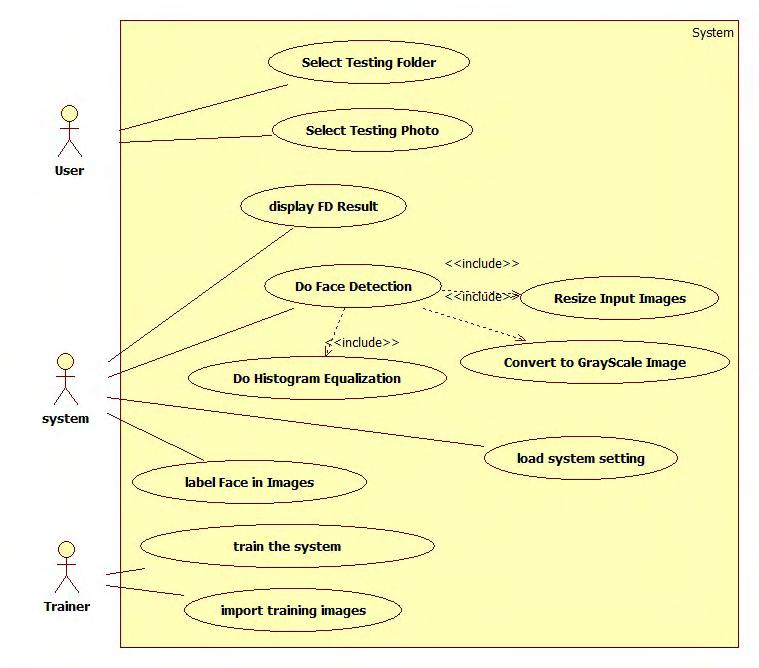
\includegraphics[width=0.9\textwidth]{Figures/UMLDrowsinessDetection.jpg}

This model is very straight forward and doesn't require to many classes like other other design frameworks for example the layered pattern which would have a downwards case layout when looked at through the unified modeling language diagram, with this type of model there isn't any loop back that can inform previous classes if an object received by the current class has been detected to have an issue which can disrupt the accuracy of the program entirely, as the data being received can be incorrect for example if camera being used doesn't identify the face and starts targeting other landmarks within the image, how would a layered model overcome this. The blackboard model will reduce the complexity of the program entirely so that a cleaner system can designed can be built.
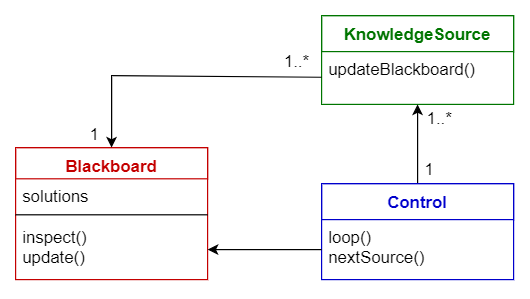
\includegraphics[width=0.8\textwidth]{Figures/Blackboard.png}
\subsection{Technologies}
A number of technologies that will be used along with this model will consist mainly of libraries and a possible external open source  technology that will be used for facial recognition. The main library that will be used will be the OpenCV and will be used for the machine learning and computer vision features that the library consists of. 
The OpenCV supports many interfaces but the interface that will be used within this system will be the python language. OpenCV has as much as 500 algorithm's that aids with real-time vision applications. The methods provided by the OpenCV such as VideoCapture() method will be used within the drowsiness detection system to access the camera and to set the capture Object as cap.read() this method will perform the process of reading each frame of the video being recorded by the camera and to store each individual frame as an image that would then be stored in a frame variable that will be created. Haar cascade classifiers may be used from this point on, the OpenCV library has methods dedicated to the use of this algorithm CascadeClassifier(‘ path to our Haar cascade XML file’) this is a process within the system that will be accompanied by a detectMultiScale(gray) this method will most likely be used to as the image will be converted in grey scale. OpenCV has a algorithm for object detection that will only take input in grey scale so when using the detectMultiScale(gray) it processes the new gray scale image that was converted from the real time image that was taken in by the camera, the detectMultiScale(gray) method is in place so that it can return an array of detection which consist of coordinates that can be plotted on an x and y axis this is all done so that the system can detect the the faces in an image and create a region of interests, this region of interest will be the eyes. 

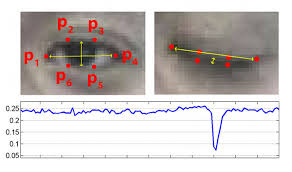
\includegraphics[width=0.8\textwidth]{Figures/eyeDetection.jpg}

The same Process will be done yet again but this time both eyes will be stored within the d method that detectMultiScale(gray) method that is within the OpenCV library. The is done so that images can be fed to the cascade classifier so that it can perform an analysis of the eye determining if the eye is open or closed. The Haar cascade classifier will run some test depending on the result of the images that it has processed internally within the algorithm and from here it can provide a score to determine if the the individual is drowsy or is not. The Drowsiness calculation is determined by a score, this score is calculated by timing how long a person has closed their eyes for. Their will be a threshold in place and the user will be alerted. 
\subsection{Database}
A back end database will be in place such as Firebase so that an administrator monitoring the drivers who are feeling drowsy can then assess the state in which the drivers are performing. A method will be used to perform continuous serialization, this is a process of converting an object into a stream of bytes so that it can be stored in a file, database or memory. Its main purpose is to save the state of the object out putted in final operation of the Drowsiness detection system so as to keep track of which current drivers are feeling drowsy and to send a personal alert to the driver to inform the driver that he is exhibiting too many instances of drowsiness and that he must take a break or otherwise he might be in danger on the road, this database will have the drivers details such as first and last name accompanied by his driver id number. Firebase stores data in real time in a JavaScript Object Notation format, Firebase database is able to perform certain functionalities such as sending an email or sending a one time code to a phone number that has been provided to the database. A simple PIP installation is required to set up Firebase database within the Drowsiness detection system, this is all that will be required so that a Firebase database implemented into the system.

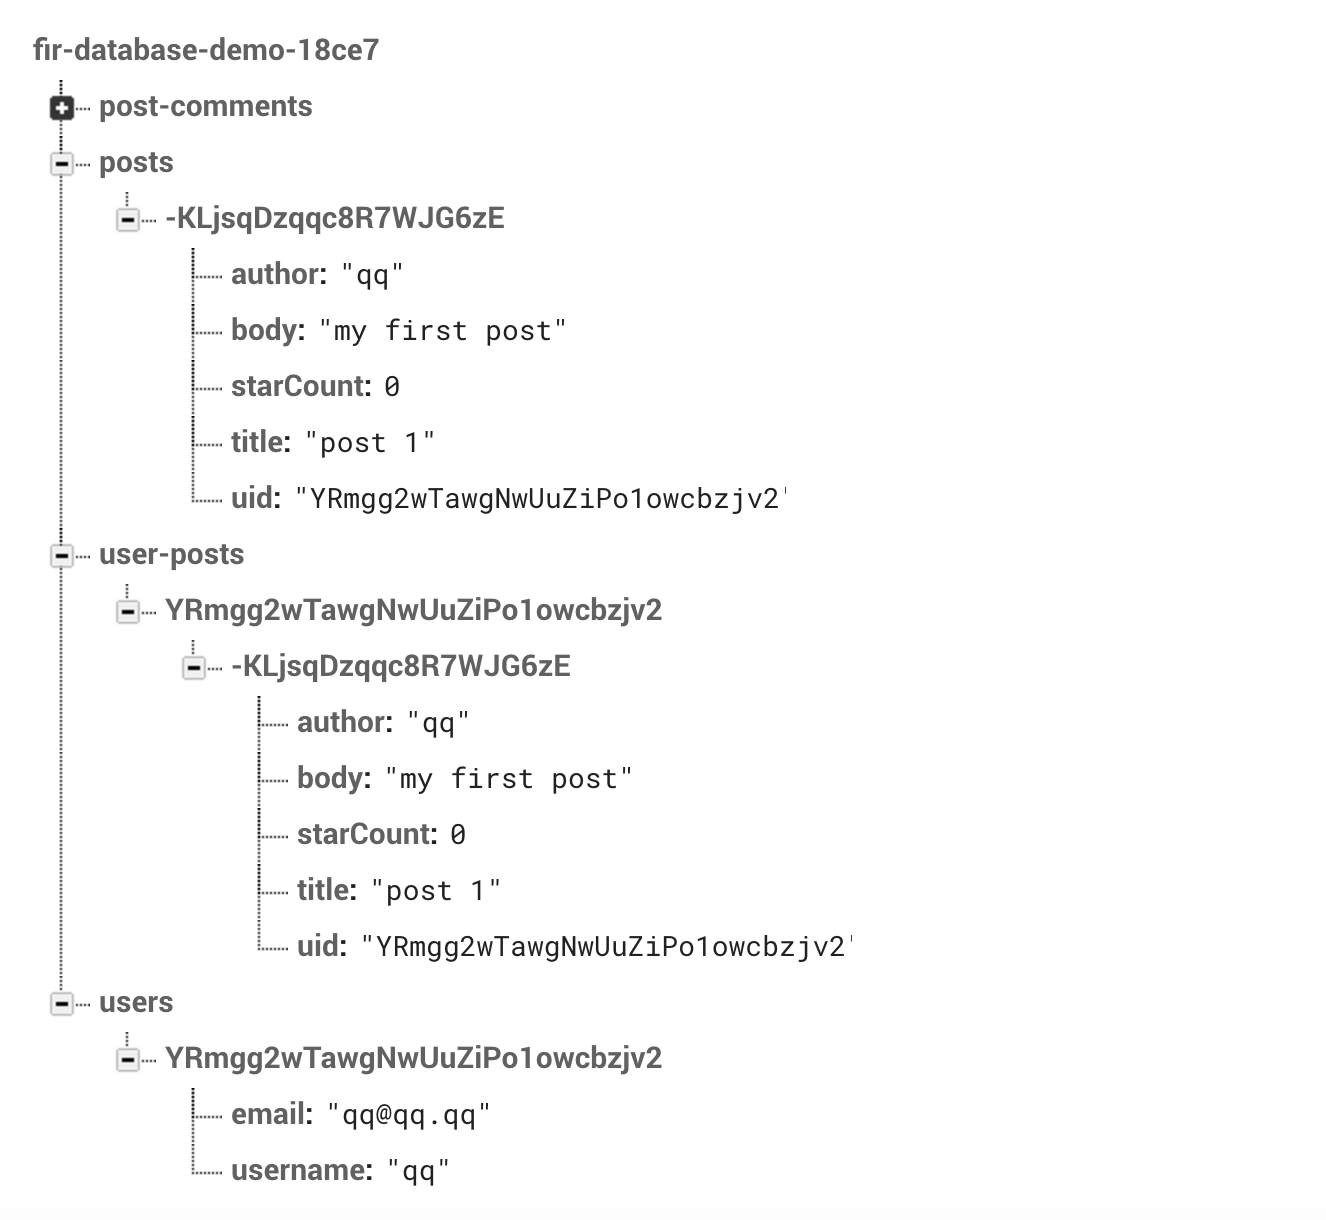
\includegraphics[width=0.8\textwidth]{Figures/Firebase.png}

\subsection{Framework}
Through this project the Python language will be used as it is commonly know as a general purpose language and accompanied by many libraries and tools that are designed for the python language most of the libraries have been detailed above that I will be using in this system.  Python is an excellent language and is the perfect choice for implementing within the architecture of this system. Python is well know for its  backend web development, data analysis, artificial intelligence, and scientific computing. When designing this system their will be a huge emphasis on artificial intelligence, with algorithms such as cascade classifiers that have to be implemented in the system these algorithms can be found inside The OpenCV library but implementing this library in python is very easy and only requires a quick import. Importing libraries into python is much more straight forward. The final design will have most likely have 4 or 5 python scripts that will communicate which each other, their will be a script Dedicated to reading the input from the camera and converting each frame to a grey scale copy which will then be accompanied by a script that will  implement Haar Cascade classifiers algorithm on the frames received of the face and the eyes, their will be a script that will then perform a threshold test that will determine if the the users is exhibiting drowsiness within the frame and then will sound an alarm if present and the final script will be a script that will perform backend database operation with Firebase database uploading the outcomes of each instance when a detection has successfully been detected and which driver triggered this. The integrated development environment that will be used to develop this system will be Pycharm as it is free has cross platform functionality and can easily integrate any backend database I require. 
This is everything I currently believe will be required by the Drowsiness detection system in term of architecture going forward 


\section{Risk Assessment }
\begin{table}[h]
\centering
\scriptsize
\caption{Initial risk matrix}
\begin{tabular}{|p{2cm}|p{2cm}|p{2cm}| p{2cm} |p{2cm}| p{2cm}|}
\hline \bf Frequency/ Consequence & \bf 1-Rare & \bf 2-Remote & \bf 3-Occasional & \bf 4-Probable & \bf 5-Frequent\\ [10pt]

\hline \bf 4-Fatal & \cellcolor{yellow!50} & \cellcolor{red!50} & \cellcolor{red!50} & \cellcolor{red!50} &\cellcolor{red!50} \\ [10pt]

\hline \bf 3-Critical &\cellcolor{green!50} & \cellcolor{yellow!50} & \cellcolor{yellow!50} & \cellcolor{red!50} &\cellcolor{red!50} \\ [10pt]

\hline \bf 2-Major & \cellcolor{green!50} & \cellcolor{green!50} & \cellcolor{yellow!50} &\cellcolor{yellow!50} &\cellcolor{red!50} \\ [10pt]

\hline \bf 1-Minor & \cellcolor{green!50} & \cellcolor{green!50} & \cellcolor{green!50} &\cellcolor{yellow!50} &\cellcolor{yellow!50} \\ [10pt]
\hline
\end{tabular} \\
\label{tab:ProjRisks}
\end{table}
As with Any system their can be many risks when first undergoing development of a system, so to for-tell if issues may arise within the drowsiness detection system we must carefully analyse all the the tasks currently understood that is required to be implemented so that a successful system can be deployed. Even though I have ensured completely that this project is carefully planned out, there is still a possibility of it running into trouble, their is always a possibility  and over the years even regardless of how I have mapped out my project work I have encountered risks that have halted my progress to completing a project with a complete and fully functioning requirements.   A  risk  in  simple way to understand  is  any  uncertain  event  or  condition  that  may  effect a developers project that has been undertaken.  However, any risk may be a scary occurrence to any developer as the developer is entering into unfamiliar territory, but not all risks are completely bad and encountering issues within a developers project can benefit the the developer in a multitude of ways for example,  one can find a  much better, easier and viable way to  implement  a certain  feature into their project,  which  can  benefit the  project and the developer.   There  is  no  guarantee that a project will be successful, so developers must be ready to handle any risk that occurs small or large. Developers learn from the risk that they faced on each project that they have taken up and have grown as engineers, becoming much more viable to their employers and the companies they work in. 
This section will detail all the possible risk that I may occur when I start the implementation face of this project.

\subsection{Hardware or software failure}
This project will be running on Lenova yoga 520 laptop with a hardware specification set with Central processing unit consisting of a Intel Pentium 4415U 140,  Graphical processing unit consisting of Intel High Definition Graphics 610 236 with a Display that is  14.0" inches, the
Lenova yoga 520 laptop has a built in camera that will be used for image processing has an internal mic and 4 speakers that will be used for sounding the alarm in the event of a drowsiness detection threshold being achieved.
\subsection{Hardware failure 1.1}
A risk that can occur in this project is that the camera or speakers that my laptop possesses fails to work when I am developing my project this issue can occur at any point during my implementation phase of this system, this is a risk that would stop my project from fulfilling  core functionality requirements within the system. This isn't the only issue that may occur in relation to hardware if a complete system failure occurs, I may lose implementation's progress and depending on which Stage I am at all my progress may be lost, progress may be lost. This may not be a common risk but I have encountered complete system failure during collage semester and project cycles. This type of risk can easily be avoided and one of the best data protections tools on the internet is to upload each bit of progress onto GitHub having a private repository in which only I have access to and where I can push each new commit, this allows for my any work done in during the implementation phase of this system to be phase and in the event of a system failure any other computer can be used to login and access my my repository and work can be continued on the system just from where I have left it before the system hardware failure. This is also the case if the Hardware failure is component based, another laptop can be used with components that are working.

\subsection{Software failure 2.1}
Another risk that may occur during the development of this is that a software failure may occur that can completely stop all my progress when it comes to developing this system, if when developing this system certain libraries that I plan on using for this project are not compatible with the hardware of my computer this can cause a major risk in the implementation phase of the system, This can be a major issue if I encounter this during development as I could have to re-decide how I will re-implement my project and can hinder progress cutting time off of the remaining time that I have left when I have to fully develop my project. Luckily when when doing my research of the technologies that I will use during for this system, everything from the languages to the libraries used are well supported and commonly used in modern applications to perform ta multitude of task so this risk is severely minimised.  If this case does happen during the implementation phase the risk wont be too great when it comes to re implementing the projects as there has been extensive research undertaken by major car organisations and fellow developers and researchers, and a multitude of different implementation techniques have been undertaken so the re-assessing time will be very minimal.
\subsection{Requirements 4.5}
Given that the development of this system is self managed by myself there is a risk of the requirements being in-adequately defined and undertaken by myself during the implementation phase of my project. During the implementation phase I may discover a requirement change or a task being unnecessary during implementation but if this happens it is possible to work around this because the core value requirement this system possesses are very difficulty to change and the likelihood of a requirement change showing up will be very rare.Their may be a decision on my end to change something about the system, and this may lack the full understanding of how how big of an impact it will have on the system.  To prevent this, good and thorough communication must be done with my supervisor and must be constant so that if any change of plan for the implementation phase needs to be designed my supervisors feedback will help me visualise this impact and if it is a good decision or isn't a good decision .
\section{Methodology}
As this is a system that will be managed by myself during the implementation phase, it is important to keep a concise list of goals that must be undertaken,  Common software methodologies such as Agile and waterfall methods during software development projects  for self-managed  projects are not typically undertaken as most  of  the  time they are in place for  team-based projects such as the the car pooling application that I have undertaken in year 3 semester 1..  The waterfall model is still used in large parts of the industries, but in many instances within the industry, it is used in combination with other methodologies, meaning its used in parallel with another very popular and commonly used model, such as Agile.  The model allows for easy a much easier testing and analysis but does not allow updating and re-implementation during the testing phase. The Agile development methodology used within the industry is a very popular approach across majority of the tech and software industries.  It is an approach that allows for adaptation and that responds to changes that are liked upon and are favorable but there are chances of deviation that can occur and this causes outcomes that are not clear. The scrum programming methodology is the methodology that I will be implementing during the implementation phase of my project with Scrum, software is developed using an iterative approach in which the team is front and center, disciplined workers on smaller teams might find the most success with this method, as it requires self-organization and self-management.

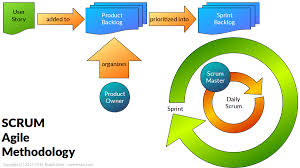
\includegraphics[width=0.8\textwidth]{Figures/Methodologies.jpg}

Team members would usually break down the end goals of a project into smaller goals so that at the beginning  of a projects they can work through them using iterations that are a  fixed length or by industry  what understood in the industry as a process called sprints to help build software and showcase it often to each other in the team, sprints usually only last  up to two weeks. Meetings play an important role in  in the Scrum approach ,and because of how the implementation phase will consist of supervisor meeting this is a very valid methodology for me to use. each sprint cycle will consist of daily planned  meetings where demos will take place to follow progress and gather feedback. Due to this, the incremental method promotes quick changes during the development cycle and adds excellent value to this complex system implementation that I will undergo. Scrum incorporates the structure and discipline of more traditional software development methodologies with the flexibility and iterative practices of modern Agile and due to this it makes scrum a very viable methodology for myself to use during the implementation phase of the drowsiness detection system.

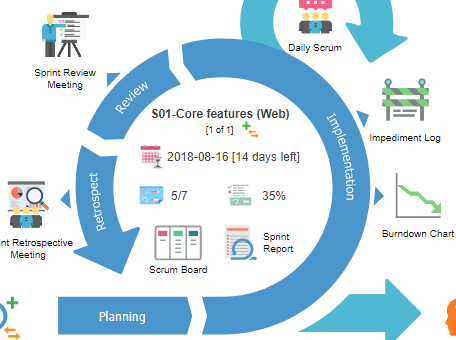
\includegraphics[width=0.8\textwidth]{Figures/Scrumchart.png}

There may be a few things that are new and need to be studied thoroughly in order to fully complete this project.  The first thing I like to do when I have encountered a new technology that I need to learn  as something new is to primarily focusing on the important sections and fundamental concepts that the new material consists of.  When it comes down to whatever it is that needs to be learned in order to complete this project. There are excellent sites that have tutorial on how to fully understand the new material that I have encountered, another important requirement of learning something new is planning and the quality of time that is allocated for it .

A good Implementation Approach of fundamentals discussed earlier when it comes to learning, is to best to choose a  environment very well suited to learning something new for example a learning environment with  no distraction. I quite room at home should be sufficient  just for learning or collage or local library would be sufficient enough when it comes to finding a suitable environment also.  It is  very important to gather a wide range of excellent resources of material that one will need to learn and to gather  so a very good understanding of the new material one must understand can be achieved. 

When trying to fulfil the Background chapter during this phase, an experienced developer will need to understand what area of Computer science the project resides within.  This requires extensive time and research as with each discipline there are a multitude of areas that must be understood, Computer Science is no different.  Firstly and  most importantly  one must  research of similar projects relating to the project at hand.  This gives a very good vision of what others have done  with projects at are within the same area that the project being researched resided in.  Having a good formulate understanding cannot be advised of one ́s project is without a doubt highly recommended, due to ones needs within the project having the ability to distinguish the differences between projects that already exist and their own project.
\section{Implementation Plan Schedule}
For the schedule I have planned during the implementation phase what I must do in the  time given to me for this project,  is to use the  duration  of  the second semester, and the time allowed to me wisely. The approach taken to make sure this project is completed is an iterative and incremental this has already been dictated by the methodologies section where I have discussed this earlier. Each of my increments we done  in equal time duration from each other.  Below I have listed all the tasks that I plan to do from the beginning to the end this should Provide the right type idea how my project implementation will be progressed from the beginning cycle until the end

\includegraphics[width=0.5\textwidth]{Figures/flowchart.png}

\begin{itemize}
\item Task 1 - Install all the required software and technologies that my system will require for example PyCharm, PyGaze, OpenCV and install Firebase into working environment.
\item Task 2 - Configure all the technologies so that my working environment has all the technologies present and running the correct version. 
\item Task 3 - Download the blackboard design model script and Begin implementing OpenCV Methods and class can work start making use of the camera components on my computer. 
\item Task 4 - Perform frame capturing functionality so to convert these frames into grey scale so that the Haar cascade classifier algorithm can start to do facial recognition 
\item Task 5 -Begin developing Haar cascade classifiers algorithm in order to use the algorithm to identify I users face.
\item Task 6 - Once developed train the algorithm start identifying a users face in each frame that is captured. 
\item Task 7 - Once the Haar cascade classifier has been trained to detect faces from each frame that is extracted of the users face then begin to train the Haar cascade classifier algorithm to detect the users eyes.  
\item Task 8 - Finally by using the Perclos algorithm to calculate the eye open to eye close ratio an score can be retrieved so that an threshold can be configured in order to detect if a user is feeling sleepy. 
\item Task 9 - Configure Alarm functionality with the speaker components on the on the computer so that when the threshold has been exhibited by the driver then the alarm will be sounded.
\item Task 10 - Begin database implementation to the system and this will be one of the final tasks to be done.
\item Task 11 -Set up JSON script inside the FIREBASE database with parameter consisting of the users details and drowsiness ratio 
\item Task 12 - Configure the serialization of data from the system to the backend database 
\item Task 13 - When drowsiness occurs with the driver then the admin monitoring the Database will be informed
\item Task 14 - Final test of the the system will be done to ensure the requirements have been met.
\item Task 15 - Provide comments and explanations of what the code does, tidy up the code in area need tidying up. 
\end{itemize}

\section{Evaluation}
When evaluating  all the goals their will undoubtedly be objectives that are achieved  quickly, while others will need some considerable  planning.  When planning is done for these tasks smaller goals can targeted allowing for the system to be developed more efficiently. These goals must  be maintained by a time bracket, this is very important in the system, Time brackets will allow the developers to measure the progress of each goal. A common approach in a project task is to simplify the task and ensure that it provides value.My final evaluation can help me learn what has been a success and what was  not  a success within this project.By understanding what this project is trying to achieve, this understanding is the core factor in understanding understanding the core evaluative measure to having a successful completion is this system come the end of next month .  To do this one I identify the project ́s objectives and they are to have a Drowsy detection system, a system that will detect if a driver is drowsy and this is done if the system can successfully detect if the user of the systems eyes are closed and this is done only when the systems algorithms and libraries are can fully extract this data from the camera on the computer. This is how i will be forming my evaluation of a successful system design design and implementation.


\section{Prototype}
Although no implementation has been done yet I carried out a few test with some of the libraries using OpenCV.

The first Test I carried out was a simple library test to see if OpenCV worked. I wrote a small script.

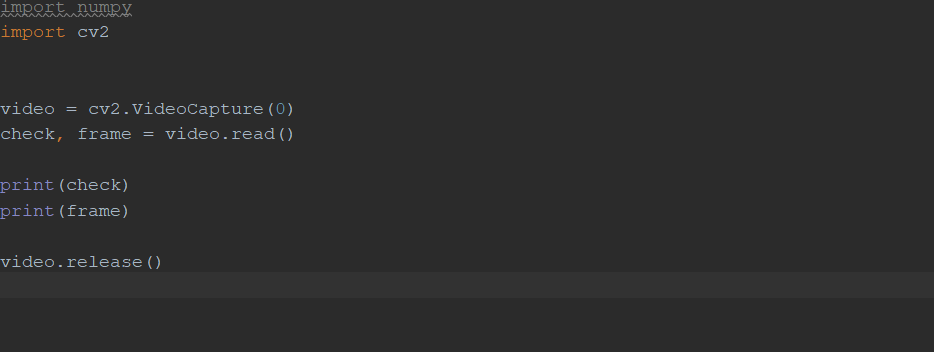
\includegraphics[width=0.8\textwidth]{Figures/Pythonscript.png}

This was the first Python script that I ran.  I ran this script so that I can observe what the terminal would output and a received what I expected from the terminal, which was matrices with zeros residing inside them. The reason They are displaying zero is because  the camera isn't active and isn't picking up any frames.

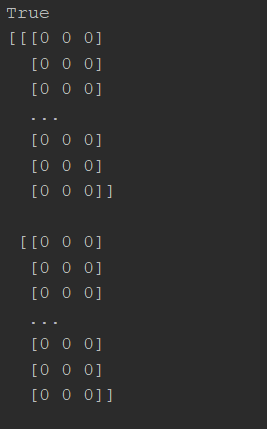
\includegraphics[width=0.8\textwidth]{Figures/terminalPythonScript.png}

This above image will show you what I the output received when I ran the script, you will see multiple matrices with zeros residing within them as i outlined before. 

I then updated my script so that I can have the camera show up on my screen although the camera is turned off by default in my setting this script shows that the OpenCV library methods are communicating with with my computer and very efficiently also.

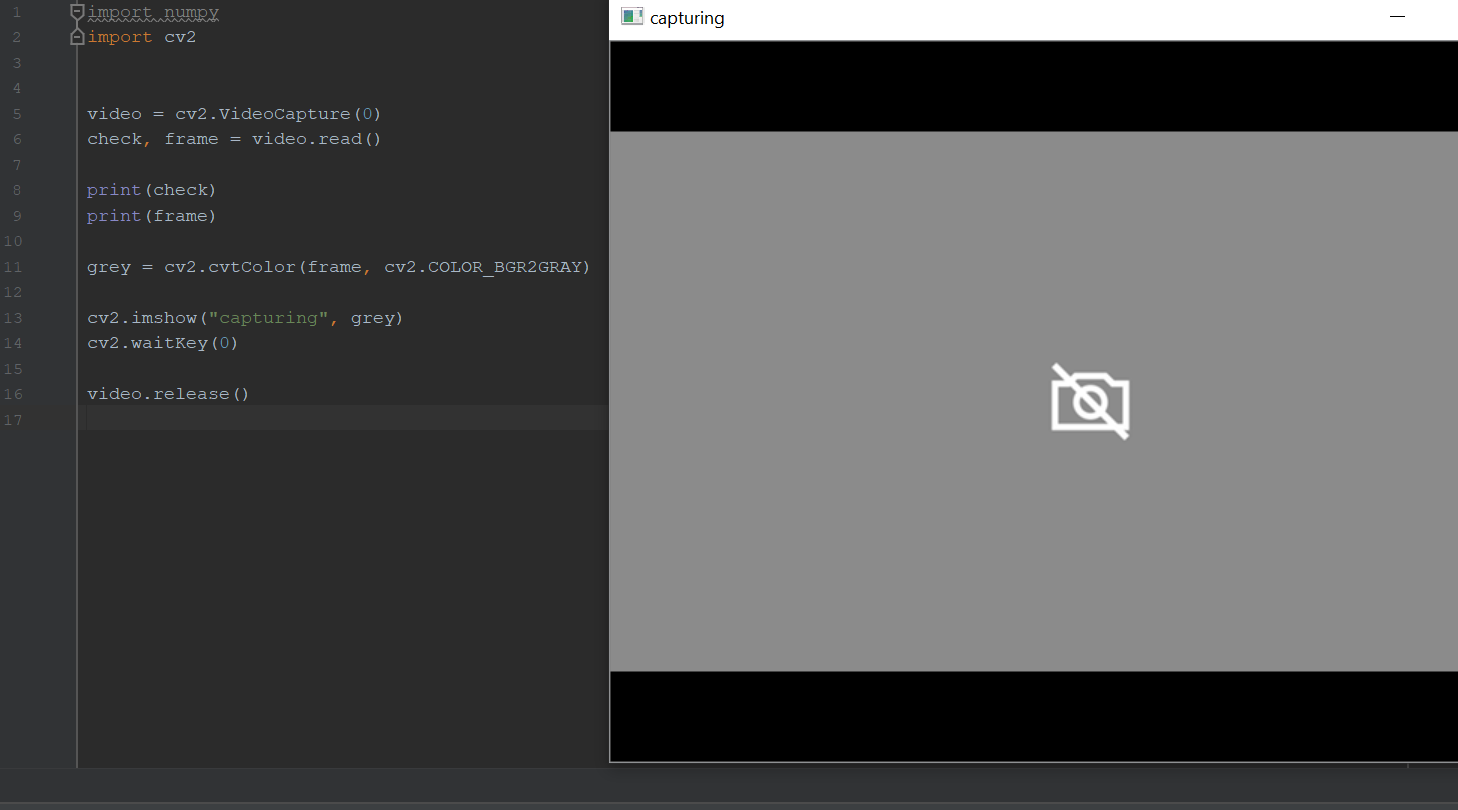
\includegraphics[width=0.8\textwidth]{Figures/Pythonscriptwithcamera.png}

AS you can see I have added a few more methods and have used a method to convert each new frame to grey scale this cant be seen as their is new picture but the functionality is within the code.




 % Solution Approach

\ifimp
\chapter{Implementation}
\label{chap:imp}
\lhead{\emph{Project Implementation}}
This chapter should comprise 15 pages and enumerate your experience when doing what you wanted to do the way you wanted to do it. 

\section{Difficulties Encountered}


 \item \textbf{Easy}
 \item \subsection{ \textbf{Camera not working } }

\item Technical difficulties where encountered throughout the implementation phase when trying to use my laptops camera in order to capture my face, this issue only occurred during the beginning of the my implementations and was easily fixed with a little troubleshooting, this issue could have been a highly fatal to the completion of my drowsiness detection system as this system is solely dependent on a working camera to capture and monitor facial features and cues from individuals exhibiting drowsiness.
  \begin{enumerate}
  \item This issue didn't have any effect on the architecture of my solution due to this being an external issue with the windows operating system.The camera wasn't updated to the latest version and was most likely clashing with the most up to date version of windows 10.
 \item This issue had a very high risk of disrupting the completion of my project as my project is very dependent on using a working camera in order to be able to perform successful facial behavioural capturing, to detect eye closure being exhibited by the individual.                                     		\item The methodology being used wasn't effected as this problem wasn't significant enough to cause any drastic methodology changes with the development of the system going forward, the only manner in which this issue may have caused an effect on the methodology that I was if this issue was in any way fatal as a complete new alternative would have to be deduced in order to progress with the drowsiness detection system. 		\item The implementation schedule was halted for a short period in order to get the camera working again, this period was significant and was majorly temporary, the implementation schedule was only halted for a week in order for me to search for a solution.                                                      
 \item The evaluation plan wasn't effected because this issue fit within the means of my project evaluation that was outlined in chapter 4, by knowing that if this issue persisted then my evaluation of a successful project would have been effected severely.															 
 \item  The first step I took when I faced this problem was to initially check if I gave pycharm permission to access my camera, when I went about ensuring if it was and then realising this wasn't the reason for the issue I then went ahead and looked at opencv forums searching for problems that other individual had that where similar to my own camera problem. I ran through these issues and they where majority coding errors, looking through these coding solutions to the the coding errors that others have experienced I copied and pasted some solutions just to check if I may have have been incorrect in my coding structure I opened a separate script to check still without any success, so from that I had deduced that is may either be a hardware issue or an issue to do with the operating system, In order to resolve this issue I found myself accessing the device manager within my computer and uninstalling and reinstalling the camera software onto my computer, then followed by a quick update, this didn't resolve my issue and I in turn found the solution by looking up the computer model and downloading the and installing the latest driver for my my camera online through google which then resolved my issue 																										
 \end{enumerate}

\item \subsection{ \textbf{Pycharm facial detection technology } }
\begin{enumerate}																																																								\item initially PyGaze was a technology that I attempted to use to capture and recognise facial cues  and behaviours, but difficulties where had trying to translate the information captured by the open source technology into information that could be understood by the python script, I then in turn switched to an open source XML import that would do the facial detection for me and could be easily understood and manipulated using python code.
\item This issue effected the design of the system slightly as I switched from open source technology to an an open source XML script.
\item The architecture was changed slightly as the open source eye tracking technology was discontinued and open source XML  was introduced which carried out all the facial, eye and mouth detection requirement
 \item It could have represented a major risk to my project if I wasn't able to find an alternative approach to the then there could have been a serious risk in the detection aspect of the system and could have resulted in a failed system.
        \item This didn't effect the methodology as I approached this problem exactly as the methodology outlined I should, by revising the my approach and taking notes of any problems and solutions to those problems 
        \item It changed the implementation schedule slightly but I remained on track as this problems solution was found and used resolve the problem very quickly.
        \item This didn't change the evaluation plan that I was using to determine successful and unsuccessful progress to the goals that I had outlined to complete.
    \item I looked open source opencv facial detection technology and quickly found a very common method that was used for facial detection systems.
    \end{enumerate}

\item \textbf{Medium}
\item \subsection{ \textbf{ Wi-Fi connection problems } }																																									\item Once my working environment was forcefully changed due to the Coronavirus all work that being done on the drowsiness detection system had to be done from home on an unreliable Wi-Fi connection, random connection losses would randomly persist and could halt any progress being carried out trying to troubleshoot errors in my code structure and logic, when good progress was being made an abrupt connectivity would interrupt that progress, connectivity loss could last up for a couple of hours and  could sometimes result in the loss of a full days work and progress.	                                                            																																                                              \item This issue was persistent and as it was evident more towards the end of the semester causing alot of the design to be implemented in a short space of time.												
\begin{enumerate}
 \begin{enumerate}
        \item The blackboard design pattern wasn't used due this issue solely as there was too many errors being displayed with its                implementation with the original solutions that I had developed initially, as well as a highly complicated structure that takes long periods of time to fully inter grate alongside my solutions for my drowsiness detection system
        \item It did possess somewhat of risk to the completion of my drowsiness detection system as there was a chance that not enough work could  have been completed before the very final deadline.
\itemThe methodologies that where outlined in chapter 4 wouldn't need to be changed due to this, the approach going forward was the same as I was using a scrum approach there wasn't any necessary need to change the methodology only to evaluate the situation and then to modify my approach implementation approach for it.  
 \item It slowed down my implementation schedule, which in turn forced me into spending less time developing the system itself this was because the window in which I could work on the system was random, although this issue happened it wasn't very frequent making it impossible to work on the system.																																														\item The evaluation plan wasn't effected because this issue fit within the means of my project evaluation that was outlined in chapter 4, if this issue persisted to the point where there was no way to to work on the system it may have effected my decision making in the evaluation of my developing the goals at the time and the final goals of the system itself
 \item In order to overcome the difficulties of this I made sure to download videos off of YouTube in case i needed to reference opencv tutorial to help achieving certain tasks that would have been required to full fill objectives and my weekly tasks, as well as taking screenshot of the OpenCV documentation using word .
   \end{enumerate}

\item \textbf{Hard}
\item \subsection{ \textbf{Caronavirus Pandemic} }																																										\item The Covid-19 pandemic was a difficulty that was encountered mid way through my project implementation, not only has this effected me but the people that I cared about around me which in turn resulted in unnecessary stress and a period of adaption. The pandemic also affected my work environment and schedule, when I had access to collage facilities the rate in which I was able to finish my drowsiness detection system was moving ahead smoothly as I had access to the collage library which had computers with a reliable internet connection, I also had access to a quite area where I could spend time performing tasks that I had planned for the week to do on my drowsiness detection system.due to the carnivorous pandemic sweeping over the world and the nation so abruptly. cases where rapidly increasing it has brought alot of uncertainty to collage progression, self isolation and environmental restriction brought into effect by the government caused for an experience that was surreal which caused panic   																																																										\item It effected the original design of the project immensely,being forced to work from home with horrible internet connections and unnecessary distractions this limited the final database functionality severely. 																																				\item It did have the biggest risk to the completion of the project because there was a high chance that I could have contracted the virus if that ever possibly happened then it could have prevented me from 	completing the system before the deadline the virus out of control and wasn't full contained by the government, although contact tracing and other procedures where carried out this wasn't enough to stop the spread.						\item It affected my weekly reviews of my progress initially until I was able to get back on track with my own weekly personal weekly reviews and overviews of the work done up the point.																																													\item It had a major effect on the implementation scheduler that I was following up until the Closure of the collages for the remained of the semester which brought on horrible connectivity issues, and an unsuitable environment to complete tasks, this took quick self adaption to get back on schedule																																																										\item The evaluation plan was slightly altered as the final system that was originally planned wouldn't be completed and I had to make do with lesser overall database functionality.																																															\item Managing the difficulty that had arisen was very difficulty to do as the Caronaviruse still  Continuous persists in Ireland and globally showing no signs of letting up, but managing other factors that where related to it such as bad Wi-Fi and bad work environment can be overcome as it is far easier to research ways to improve your work environment or to call the internet service provider in order to fix issues with the connection by bringing it to there attention.
\end{enumerate}
	


\section{Actual Solution Approach}
In December of last year, when writing the first version of the report, in Chapter 4 you came up with your original solution approach. On it, you presented (i) the architecture of your solution, (ii) your list of use cases, (iii) a risk assessment, (iv) a methodology to develop your solution approach, (v) your implementation schedule, (vi) your evaluation plan and (vii) some prototype of the resulting product. From January to April you have been developing your solution approach. Along the way you have encountered difficulties (the ones listed in Section 5.1) which might have modified your original plan so that you can come up with an actual developed project.

This section is effectively the production of "as built" specification where you compare your original design to the final finished project. Please go section by section (the ones listed from (i) to (vii) in the last paragraph. For each section, enumerate any difference between the original design and the final project, and justify the difficulty forcing you to make such this change. Do not fret if some of these changes are radical, what is important here is that there is a clear rationale for changes made.
[By the end of December of last year I had an initial understanding of the opencv library and a basic understanding and design of the architecture that  I thought was enough to successfully to build the drowsiness detection system, some design outcomes in the research phase have been used in the implementation phase which is a sign of good research carried out previously and some outcomes that where researched and found to be of no use within the final implementation build, overall I will be detailing my progress through the implementation phase and comparing the final solution to the research phases architecture and final conclusions, both overall outcomes will be compared under a number of factors, like architecture ,use case , methodology , implementation schedule, evaluation plan and prototype,  all these will be the premise from which I will be detailing my solution approach

\subsection{Solution Architecture}
\subsection{Design Model}
During the research phases I specified my architectural specification of the drowsiness detection system I said I would be modelling the system using a blackboard design pattern, however when developing my system I had issues  implementing this design pattern as it was too complex for the time required, choosing this design model  at the time suited the type of system that I was designing  as it suited the needs of the system as it was heavily recognition focused. The blackboard design pattern would typical be used solely for speech recognition but when it came to developing my drowsiness detection system I intended to use it for the for the user identification aspect of the system.  When designing the solution I initially attempted to fit the  blackboard skeleton into my code but encountered issues when it came to capturing a new frame and storing it as an image in a directory in order for the system recognise the individual from the image. 

\subsection{Technologies}
When I first did my research on the  technologies that I would have been using in the the development phase my research was very accurate as almost all the technologies where used.When i was developing the system I had to use other technologies within the project itself to successfully achieve the goals and ambition that I had going forward. The main library that was used in the solution approach was the OpenCV and this library was essential in carrying out facial detection, video capturing and facial recognition in the project. The interface that the OpenCV was used with was the the python language this was specified in chapter 4, methods that where specified in where used to do exactly as was specified within the research phase, methods like the VideoCapture and read() where both utilized thorough out the development of the drowsiness detection system .
 Haar cascade classifiers where used to detect the face and eyes of the individual, there where multiple unique types of harrcascade scripts that performed different types of detection these scripts where used simultaneous, parallel to each other in order to perform eye detection face detection and detection when glasses where on the individual, during the implementation i used methods dedicated to reading Haar cascade files OpenCV had a built in algorithm called CascadeClassifier that would access the cascade file using CascadeClassifier(‘ path to our Haar cascade XML file’)  this process within the system was always accompanied by a detectMultiScale(gray) this was used to perform grey scale capture as the computer processor can only differentiate  shades of darkness, the detectMultiScale(gray) method is in place so that it can return an array of detection which consist of numerical values that are plotted on an x and y axis without the capture being converted to grey scale the computers processor wouldn't be able to detect differences in in each frame this is all done so that the system create a region of interest.
 

\subsection{Database}
A back end database was one of the intended functionality requirements to be in place when the research concluded in December, Firebase  was the database that was decided upon to add backend administrative functionality to the system the idea was to have an administrator monitor over the drivers and to detect if the driver was sleepy and showed signs of drowsiness, assess the state in which the drivers was performing on the road.  The purpose of the database was to save the state of the driver in order for it to be referenced by the Drowsiness detection system so as to keep track of which current drivers are feeling drowsy and to send an alert to the driver to inform the driver that he is exhibiting too many instances of drowsiness and that he must take a break or, goal of the database was to have all the details that where unique to the driver  such as first and last name accompanied by his driver id number. In the final system i was only able to capture the number of times a driver was feeling drowsy and to upload it to the database, this is far from the database functionality that was envision in December this lack of database functionality was mostly due to the covid-19 pandemic that altered and slowed down the development schedule.

\subsection{Framework}
In December I decided upon Python as the language that will be used as it was commonly know as a general purpose language and was accompanied by many libraries and tools that are designed for a wide range of unique projects. The usefulness of Python was evident as an excellent language and was the perfect choice for implementing  architecture of this system. Python is well know for its  backend web development its artificial intelligence and the scientific computing frameworks is possesses, as I designing this system their was huge emphasis on artificial intelligence the haar cascade classifiers scripts that where used to detect a face being displayed in the webcam,  implementing  these scripts where easy, opencv has methods which support external cascade XML imports.  The final design consists of  a single python scripts that will communicate  with multiple haar cascade XML imports which each other, their is  multiple methods Dedicated to reading the input from the camera and converting each frame to a grey scale copy which is then be accompanied by a script that reads and implement Haar Cascade classifiers algorithm on the frames received of the face and the eyes, their is a method that implements a cascade file which detects a if individuals has blinked which is then proceeded with an alarm. 

\subsection{Hardware failure 1.1}
A risk that did occur in this project was an initial hardware failure that was the camera not working initially preventing   halting initial work  trying to develop my project  if this issue persisted during my implementation phase of this system, it presented a risk that would stop my project from being fulfilling  the  core functionality requirements of the system thankfully this issue was resolved and i was able to progress with developing my system. This was an  issue touched upon in the research phase as I said if this occurred in relation to  their being a hardware failure their could be a high possibility of a  complete system failure occurring, loss of  implementation's progress was also stressed and depending on which Stage i was at I  could have lost all my progress. This wasn't a  common risk but a very reasonable on and this predictive thinking helped  insure a  there wasn't a complete system failure during the collage semester and through out the implementation. This type of risk was easily avoided by the use of  GitHub allowing me to commit each work cycle  in the event of a system failure any as if this happened i could access me work  using any other computer to access my my repository and work can be continued on the system where I have left it before the system hardware failure.

\subsection{Software failure 2.1}
Another risk that did occur during the development was a software failure which required a change in design from a eye tracking open source software to a XML import file to continue  my progress to developing the system, if I perhaps couldn't find an alternative then developing this system would have failed, in December i predicted that certain libraries I planned on using for this project may not have been compatible with the hardware of my computer but in actuality it was the open source eye tracking technology that caused the issue and if this issue persisted then a major risk in the implementation phase of the system was evident, ""\textbf{This can be a major issue if I encounter this during development as I could have to re-decide how I will re-implement my project and can hinder progress cutting time off of the remaining time that I have left when I have to fully develop my project}"" these are the exact words that I used in  the case this happened through the implementation phase . Luckily when doing my research i had found multiple directions I could have taken to fully complete the this assessment and when my initial direction didn't work I changed to an alternative method which took a little longer to grasp and implement . 
\subsection{Requirements 4.5}
As the development of this system was self managed by myself there was risk of the requirements being in-adequately defined and undertaken by myself during the implementation phase of my project. During the implementation phase I discovered a requirement changes and functionality additions such facial recognition using in built facial trainer and instances where tasks became unnecessary due to time constraints such as a backend database during implementation when this happened work around where though of and implemented such as to equal the weight of functionality lost for the removal of a database, facial recognition was added as a counter balance because this core  requirement  change in this system produced  difficulty. Requirement change wasn't expected to show up in December, my expectation of this was very rare at the time but this is now not the case .Their was decisions made on my end to change functionality of the system, and this came down to lack of time forcing drastic changes which has had a big impact on the  the system. 
\section{Methodology}
The waterfall model was used as It was the most popular development methodology when researched upon and used in large parts of the industries,  it is used in parallel using an agile technique.  The model allowed for far easier testing  and analysis through out the development of my system. The Agile development methodology used to continually allocate my work into a cycle and to continuously evaluate successful sprints at the end of each cycle, i allocated myself mostly a week to perform each task that i had in my schedule and in the case it took longer at the evaluation phase i would then proceed allocate more time in the next sprint to accomplish the previous task and the following task.   It was an approach that I found  suitable  for adaptation through out development of the system. The implementation of this methodology allowed  for adaption in the later stages of developments change deviation at these stages can be damaging  that can occur and but the time heavy cycles can create opportunity to implement other functionality this caused the  outcomes not to be clear. The scrum programming  methodology is the methodology that I used to implement functionality, each iteration is a cycle of one week self management and organisation is needed and this made the scrum suitable through out the development system
  

\subsection{Implementation Schedule}
This was the schedule I  planned  and followed during the implementation phase within the research phase,  is to use the  duration  of  the second semester, and the time allowed to me wisely. The approach taken to make sure this project is completed is an iterative and incremental this has already been dictated by the methodologies section where I have discussed this earlier. Each of my increments we done  in equal time duration from each other.  Below I have listed all the tasks that I plan to do from the beginning to the end this should Provide the right type idea how my project implementation will be progressed from the beginning cycle until the end

\begin{itemize}
\item Task 1 - Install all the required software and technologies that my system will require for example PyCharm, PyGaze, OpenCV and install Firebase into working environment.
\item Task 2 - Configure all the technologies so that my working environment has all the technologies present and running the correct version. 
\item Task 3 - Download the blackboard design model script and Begin implementing OpenCV Methods and class can work start making use of the camera components on my computer. 
\item Task 4 - Perform frame capturing functionality so to convert these frames into grey scale so that the Haar cascade classifier algorithm can start to do facial recognition 
\item Task 5 -Begin developing Haar cascade classifiers algorithm in order to use the algorithm to identify I users face.
\item Task 6 - Once developed train the algorithm start identifying a users face in each frame that is captured. 
\item Task 7 - Once the Haar cascade classifier has been trained to detect faces from each frame that is extracted of the users face then begin to train the Haar cascade classifier algorithm to detect the users eyes.  
\item Task 8 - Finally by using the Perclos algorithm to calculate the eye open to eye close ratio an score can be retrieved so that an threshold can be configured in order to detect if a user is feeling sleepy. 
\item Task 9 - Configure Alarm functionality with the speaker components on the on the computer so that when the threshold has been exhibited by the driver then the alarm will be sounded.
\item Task 10 - Begin database implementation to the system and this will be one of the final tasks to be done.
\item Task 11 -Set up JSON script inside the FIREBASE database with parameter consisting of the users details and drowsiness ratio 
\item Task 12 - Configure the serialization of data from the system to the backend database 
\item Task 13 - When drowsiness occurs with the driver then the admin monitoring the Database will be informed
\item Task 14 - Final test of the the system will be done to ensure the requirements have been met.
\item Task 15 - Provide comments and explanations of what the code does, tidy up the code in area need tidying up. 
\end{itemize}

\section{Evaluation }
 At the end of my development my evaluation had changed as  some of the goals that i had and objectives where changed, what was achieved  quickly was evaluated and noted by the successful output of the system, while others objectives need  some considerable  planning to develop work around that where considered sufficient  evaluated outcomes .  When  i performed my planning  for these tasks to be developed evaluation conditions had to be implemented along with them to have efficient outcomes. These goals where maintained by a time bracket as was specified  by the scrum the time bracket allowed me to measure the progress of each goal, simplification of the task ensured that it provided easily understood value. My final evaluation can be seen as a success as the main core functions have been achieved the evidence is the alarm being triggered when my eyes are closed and what was  not  a success within this project such as  the database  is evident because database functionality is missing .By understanding this i understood what i wanted to  achieve, this understanding was the core  evaluation factor i needed to perform my evaluative measure to having a successful outcomes at the end of my development. Other evaluation techniques where used to determine if the system was doing tasks correctly such as threshold the detection  parameters to suit the needs of the the system efficiently.


\section{Prototype}
Although no implementation has been done yet I carried out a few test with some of the libraries using OpenCV.

The first Test I carried out was a simple library test to see if OpenCV worked. I wrote a small script.

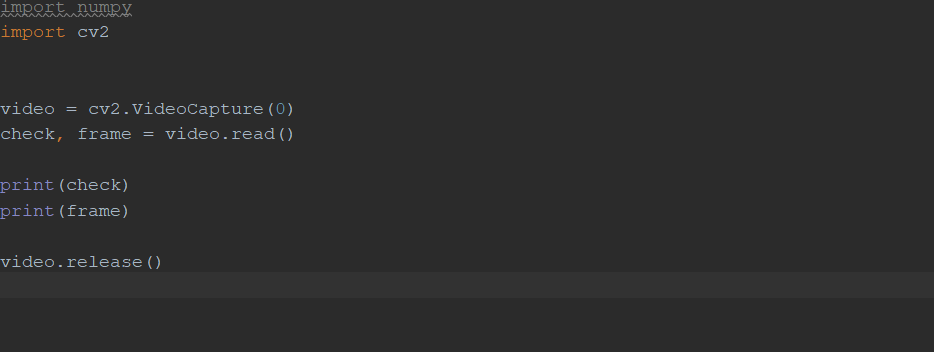
\includegraphics[width=0.8\textwidth]{Figures/Pythonscript.png}

This was the first Python script that I ran.  I ran this script so that I can observe what the terminal would output and a received what I expected from the terminal, which was matrices with zeros residing inside them. The reason They are displaying zero is because  the camera isn't active and isn't picking up any frames.

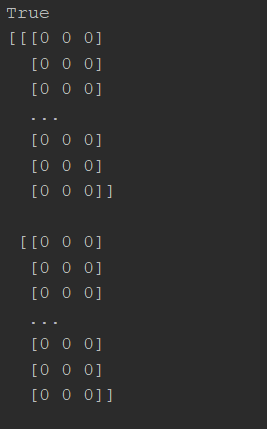
\includegraphics[width=0.8\textwidth]{Figures/terminalPythonScript.png}

This above image will show you what I the output received when I ran the script, you will see multiple matrices with zeros residing within them as i outlined before. 

I then updated my script so that I can have the camera show up on my screen although the camera is turned off by default in my setting this script shows that the OpenCV library methods are communicating with with my computer and very efficiently also.

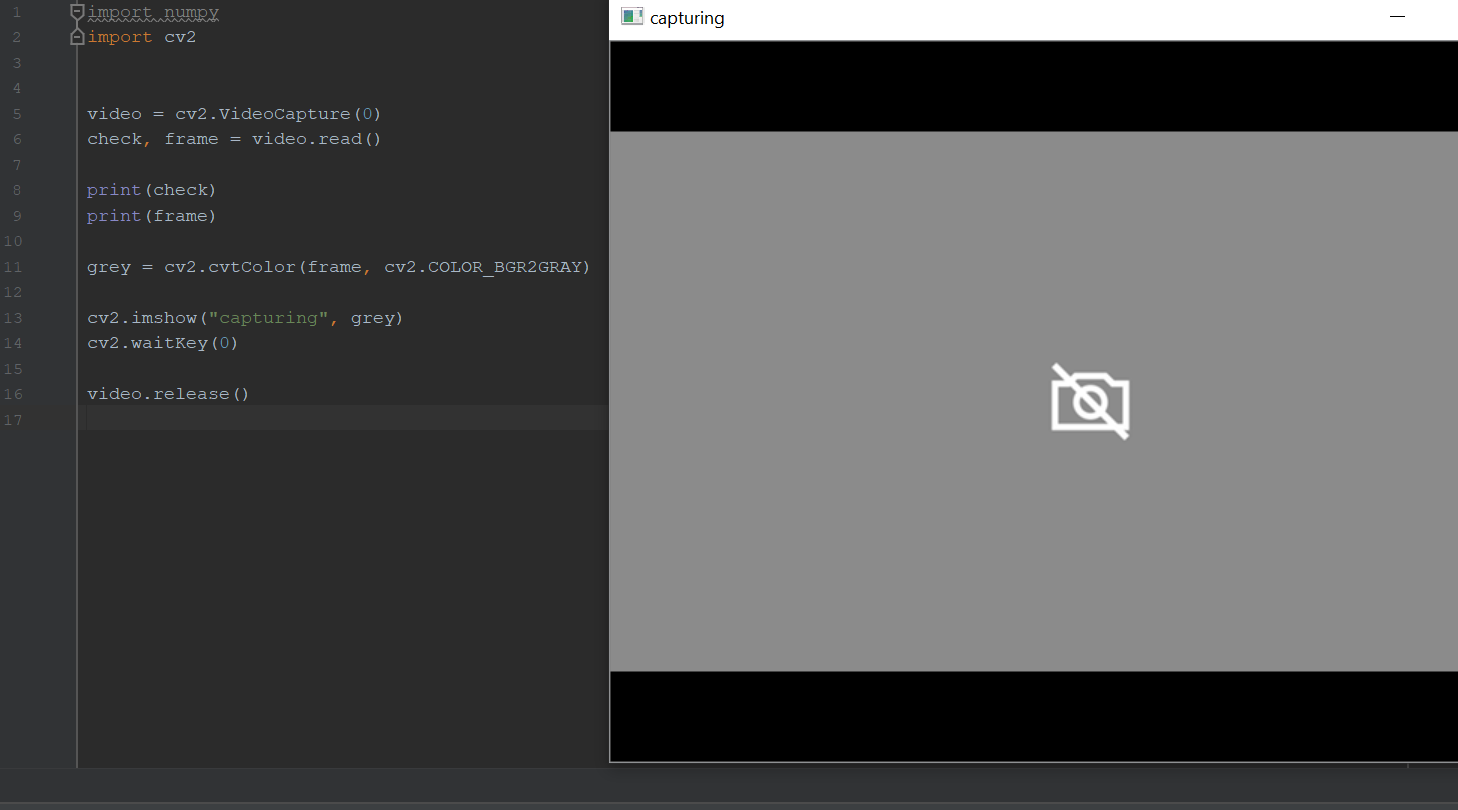
\includegraphics[width=0.8\textwidth]{Figures/Pythonscriptwithcamera.png}

AS you can see I have added a few more methods and have used a method to convert each new frame to grey scale this cant be seen as their is new picture but the functionality is within the code.

]
















 % Conclusions and Term 2 work
\chapter{Testing and Evaluation}
\label{chap:eval}
\lhead{\emph{Project Testing}}
\usepackage{graphicsx}
The goal of this chapter is an objective evaluation of the final system. The evaluation must be quantitative and not qualitative. You may perform qualitative evaluation but this should not form the basis of the main conclusions you derive from the evaluation. This evaluation, where possible, should be comparative, i.e. you should evaluate your system against a commercially available system and/or system detailed in a research publication. You should demonstrate operational testing of the project using real or contrived data sets to evaluate aspects of the project not encompassed in the software testing (e.g. quantify how well does your project achieved the overall goal). 
\begin{itemize}
    \item For software based projects this will include, but should not be limited to, evaluation of non-functional requirements.
    \item For infrastructural projects this testing should include system/network KPI analysis.
    \item For analysis based projects (ML, malware or other) this may include model evaluation or YARA rule validation, for example.
    \item For management projects, where software testing or infrastructure testing may not be in scope, the test process for the system is expected to be more rigorous and well described than a project incorporating significant development work.
    \end{itemize} 
When Testing this system I conducted a select few test to ensure that this system performed the select number of tasks that was required for accurate detection of the individual.



\section{Metrics}
Identify and describe the metrics you used to evaluate your project. You should have identified some of these in the research phase report but will detail these as you progress through the design.
When Testing this system I conducted a select few test to ensure that this system performed the select number of tasks that was required for accurate detection of the individual.
1)   camera testing and haar cascade testing
2)   Testing of the haar cascade files
3)  facial recognition and identification testing through video    . 
4)   Complete system test to ensure that all components ran together and performed accurate facial detection.
It is important to note that the system is designed in a manner in which one set of functionality is added upon the previously built functionality.

\section{System Testing}

\subsection{Camera testing and video capture analysis }
The most effective method for camera testing  is to run a simple script  to activate the camera from within the pycharm working environment, along with this it is best to print put the frame which is capturing the video. A Simple script can be run to determine  if  all the opencv's packages have been installed  and imported into the working environment. 



\begin{figure}[h]
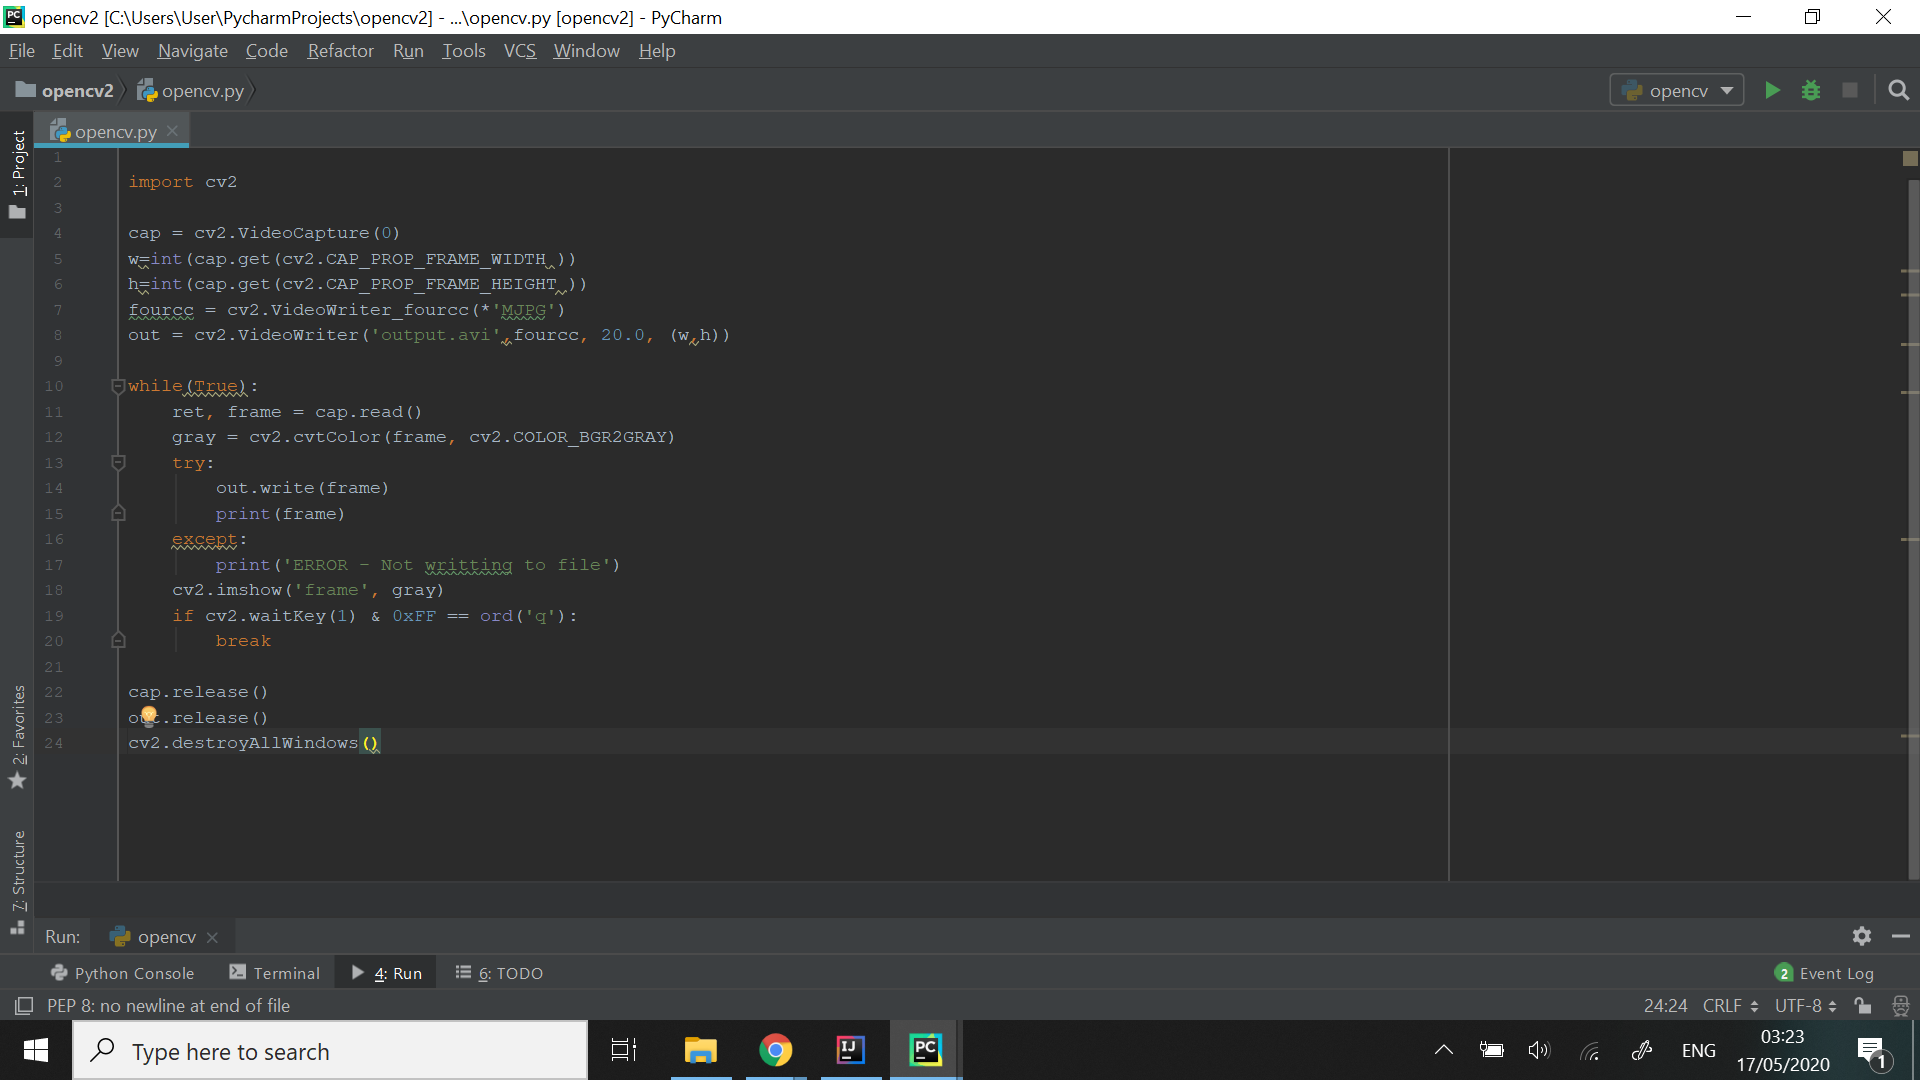
\includegraphics[width=0.5\textwidth]{Figures/videoScript.png}
\end{figure}



As you can see in the image below there is a active camera with actual video being ran of the back ground,This proves to me that opencv's packages are correctly imported into the project and is working 

\begin{figure}[h]
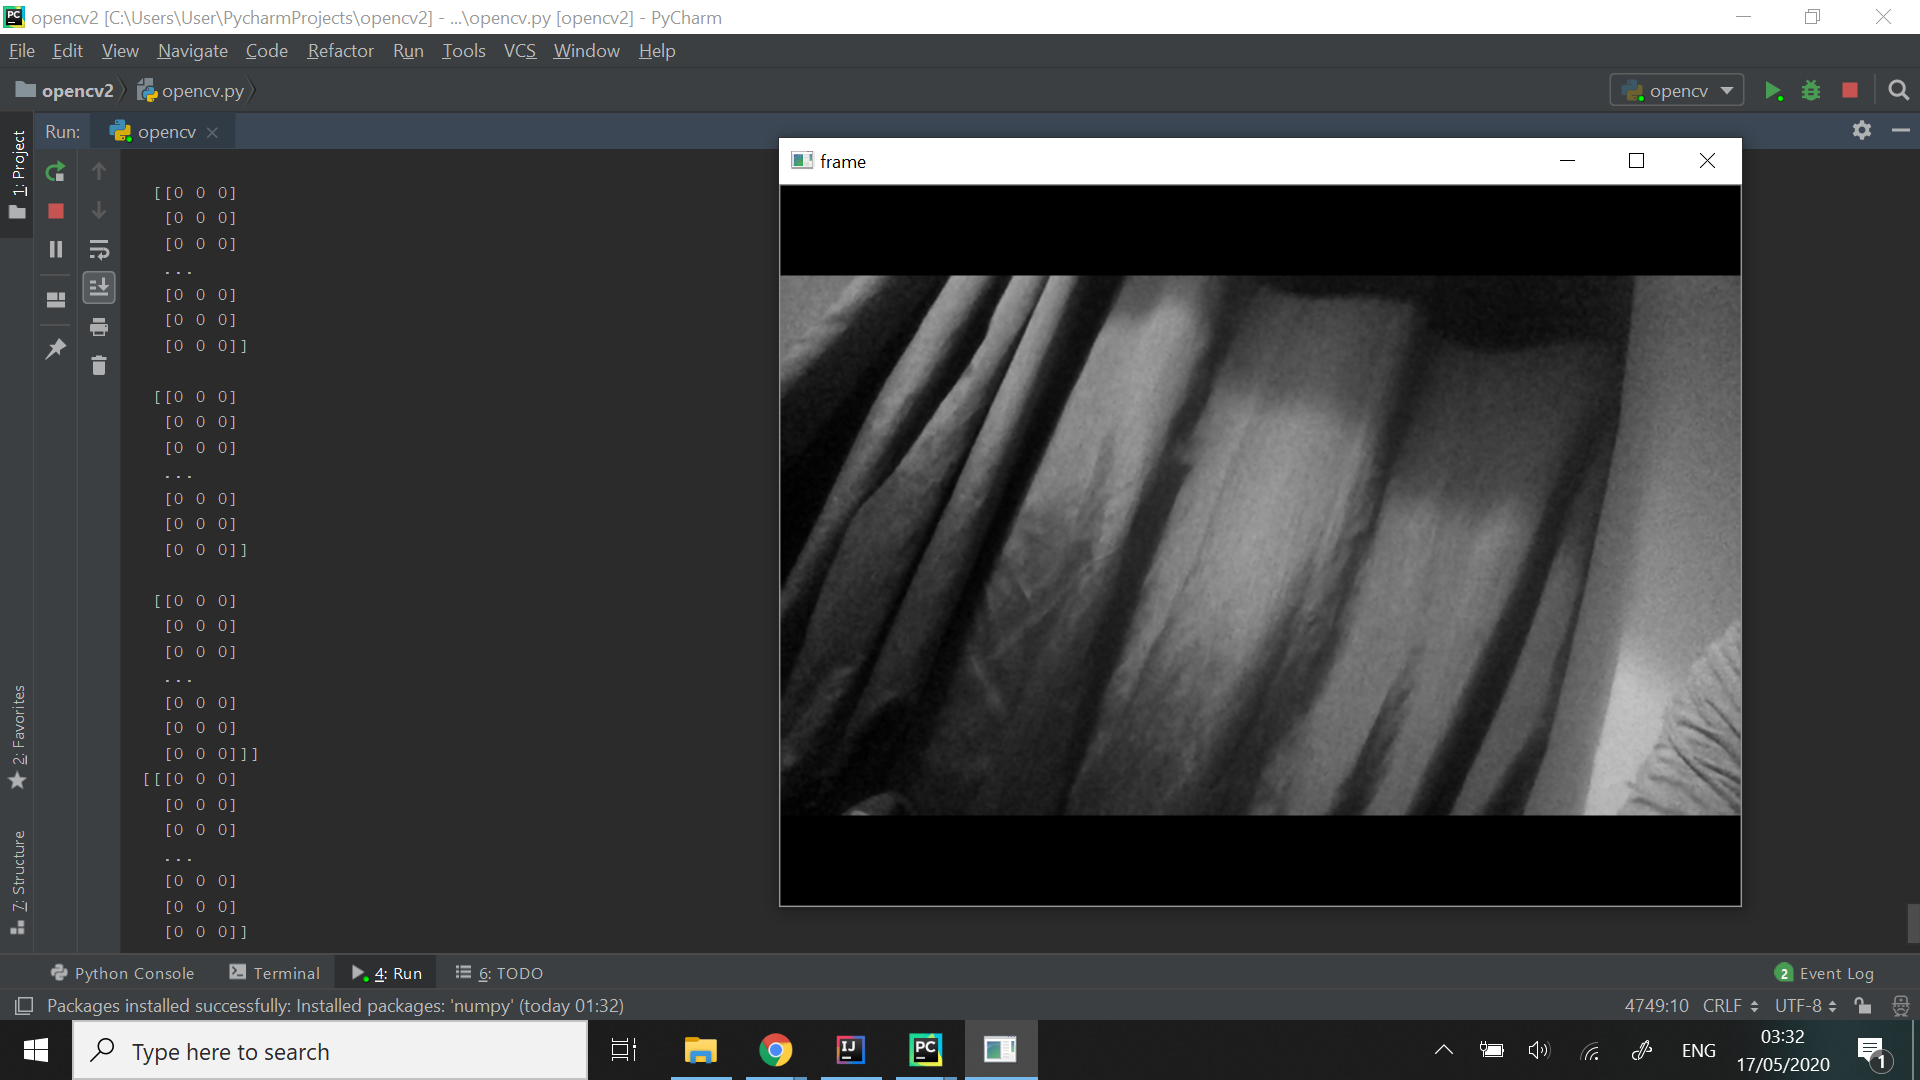
\includegraphics[width=0.7\textwidth]{Figures/video capture.png}
\end{figure}


As the opencv is configured correctly, video analysis can be done now and to perform this we need to be sure that what is being captured is being understood, the easiest way to test this is by having your script print out the values that are stored in the frame, doing this is very straight forward as you can see in the above image to the left of the video you can see that there is a matrix being printed out with the value that is being streamed into the frame. at the moment its all zeros which means nothing is being recognised by the processor. 
\begin{figure}[h]
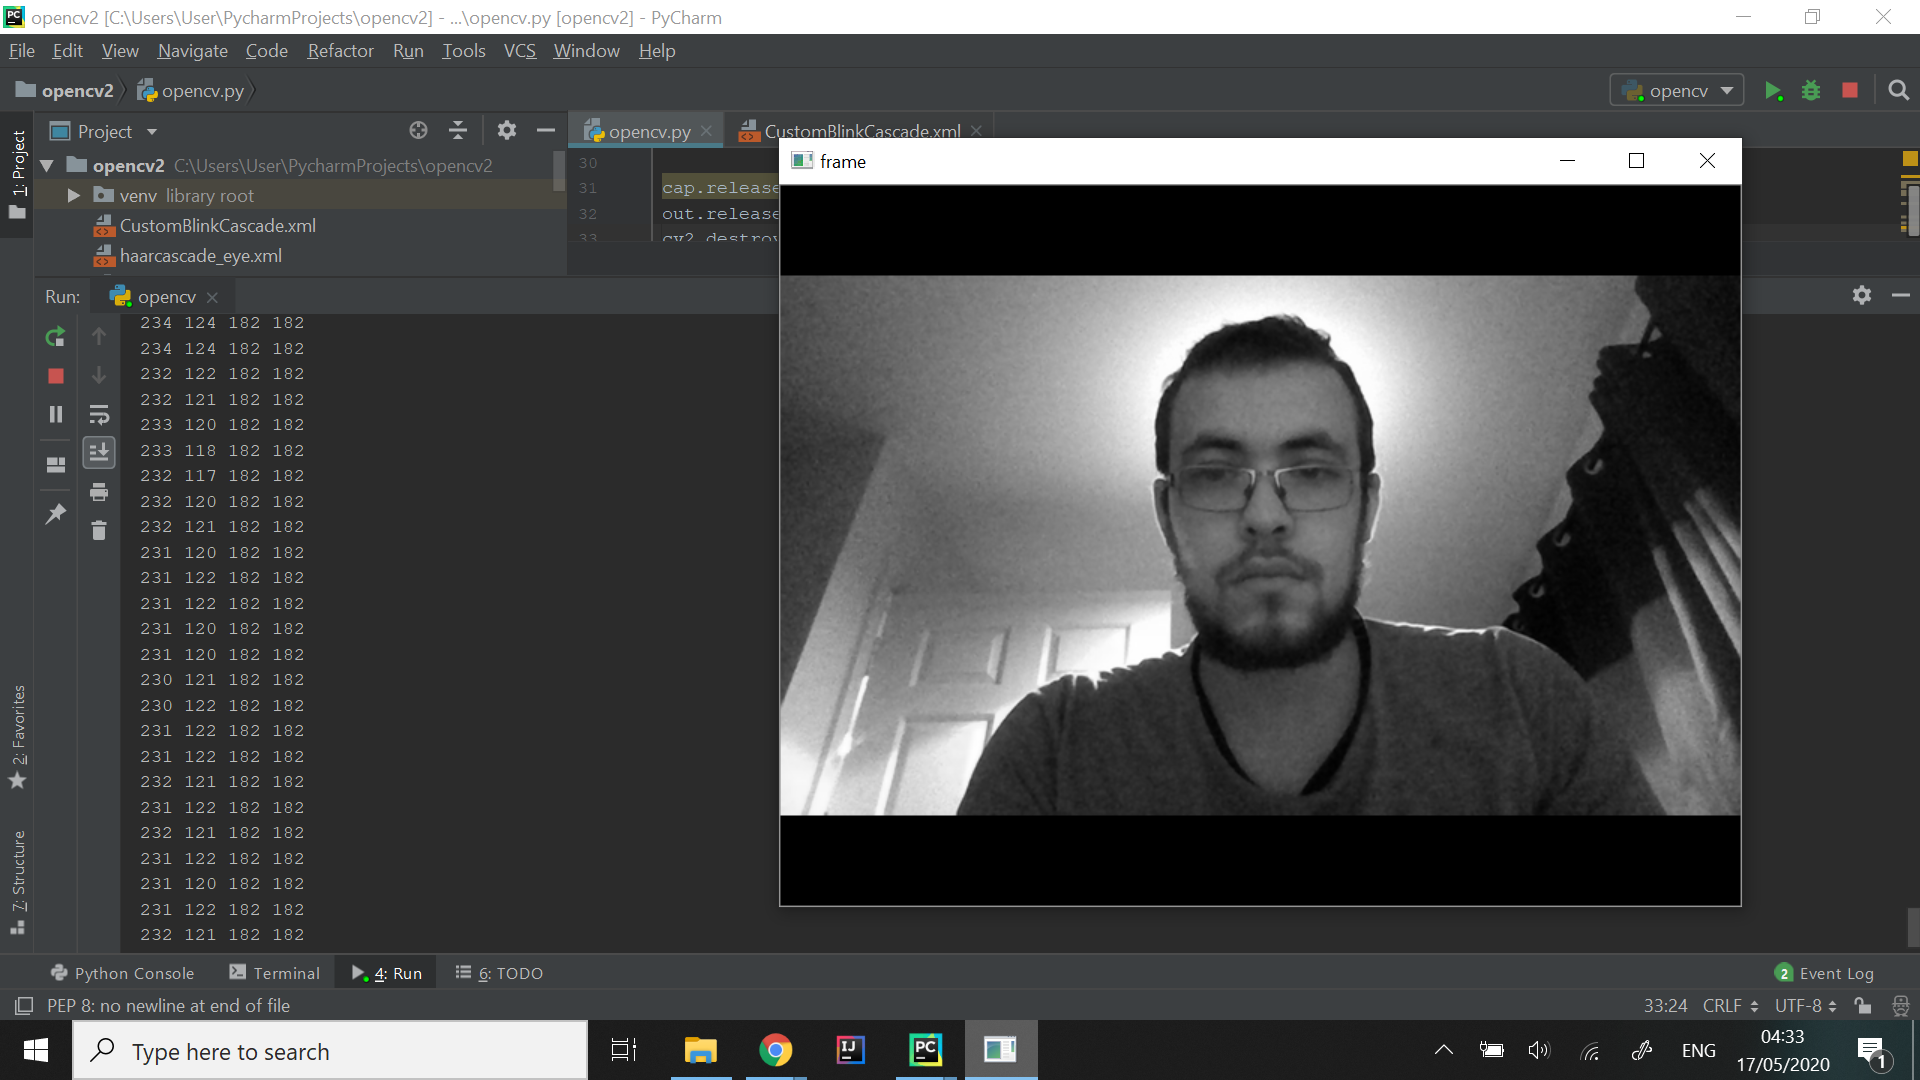
\includegraphics[width=0.8\textwidth]{Figures/videoanlysis.png}
\end{figure}
The above image show myself and beside it the matrix with validates the analysis, you can see that in previous images there was the value zero within the whole matrix and when video is analysing my face you can see that the value being printed within the matrix of myself is an infinite stream a numbers that represents me in the background of the video.
 
\subsection{Testing of the haar cascade files}
in order to test if the haar cascade files are accurately detecting my face i need to set up a test in which i must use the matrix to and python geometry to create a box around my face if the boy isn't present around my face then i can assume with great accuracy that my face isn't being detected by the haar cascade XML file. I build a script to test this.   
\begin{figure}[h]
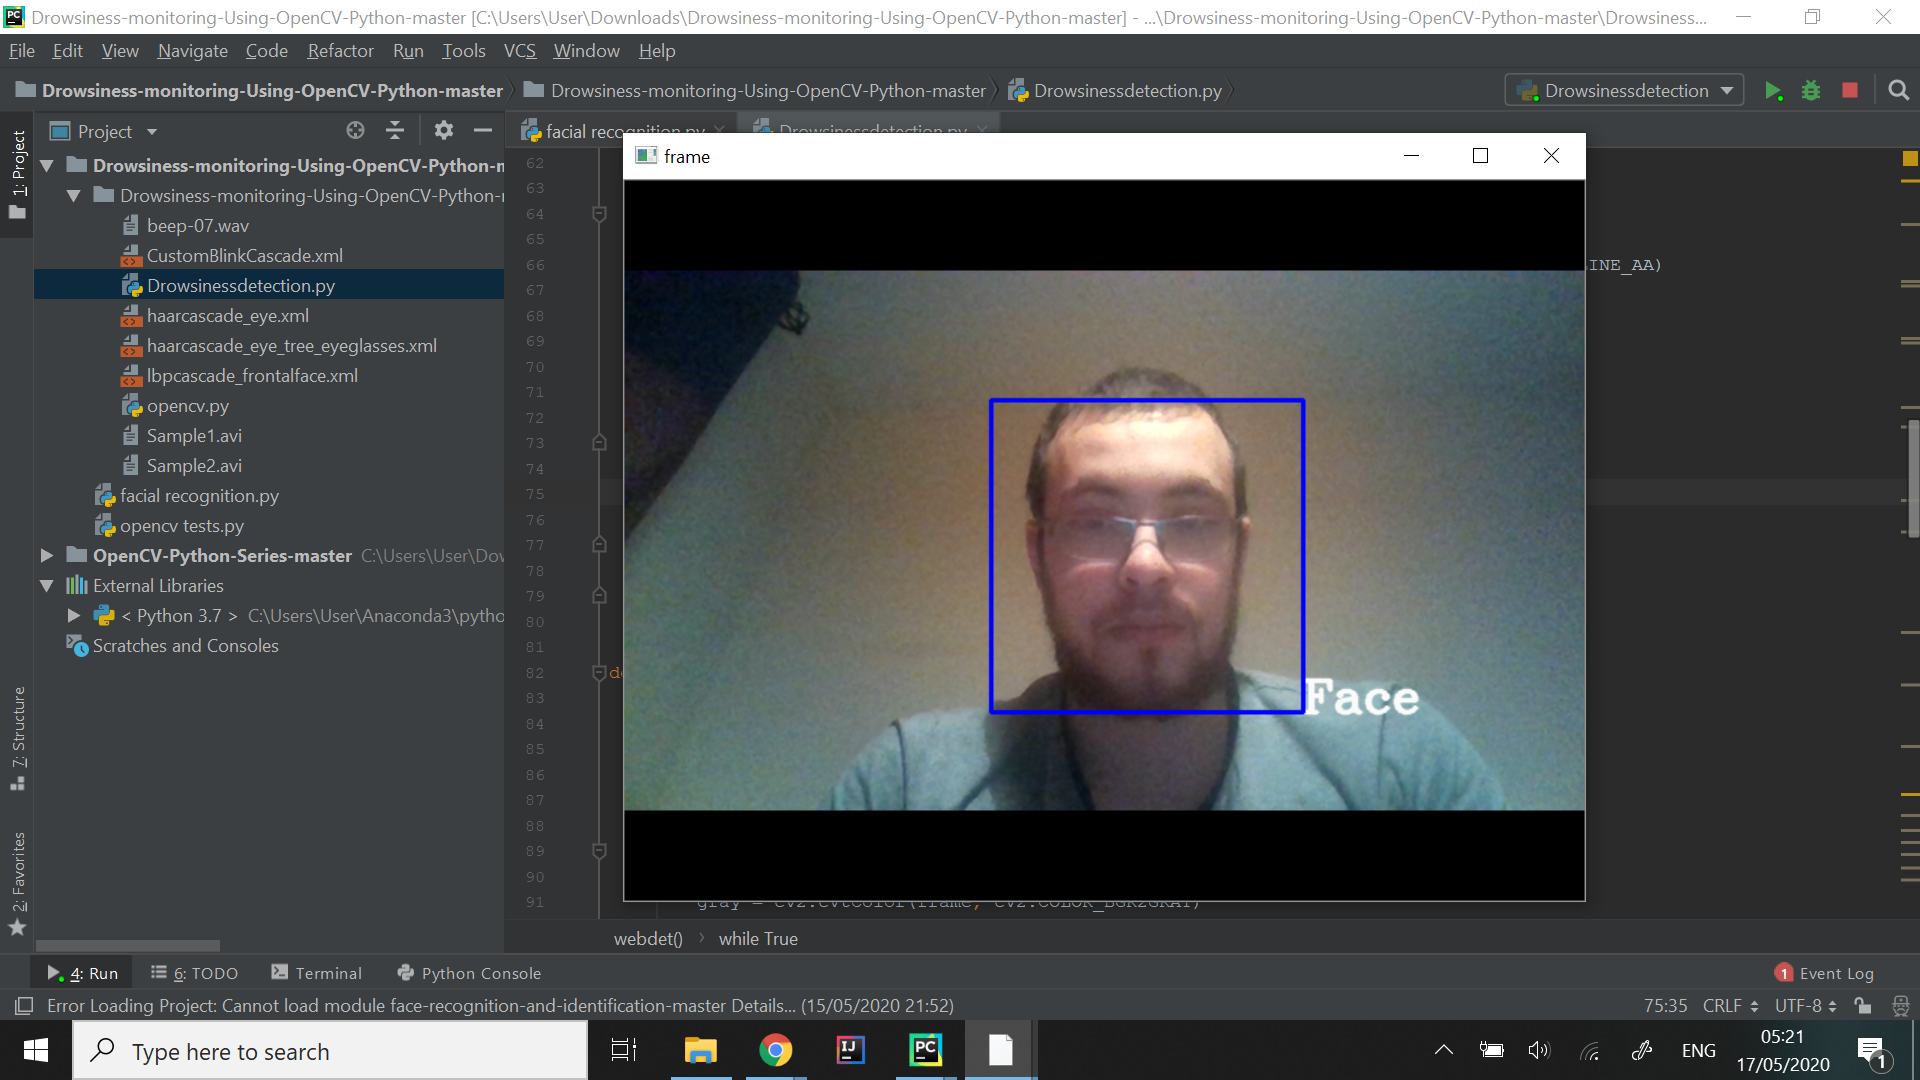
\includegraphics[width=0.8\textwidth]{Figures/facedetect.png}
\end{figure}

As you can see in the image above a blue box outlines my face which means that the haar cascade file is implemented correctly there is also a label beside it which tells me that rectangle has detected my face. The code that is highlighted is the block of that determined the face location in the video and displays a box around it. This is done by taking an x-y coordinate and setting the size of the rectangle equal to the size of the detected face that can only be detected using the cascade this then validate my test for the haar cascade being implemented properly and working 
us\begin{figure}[h]
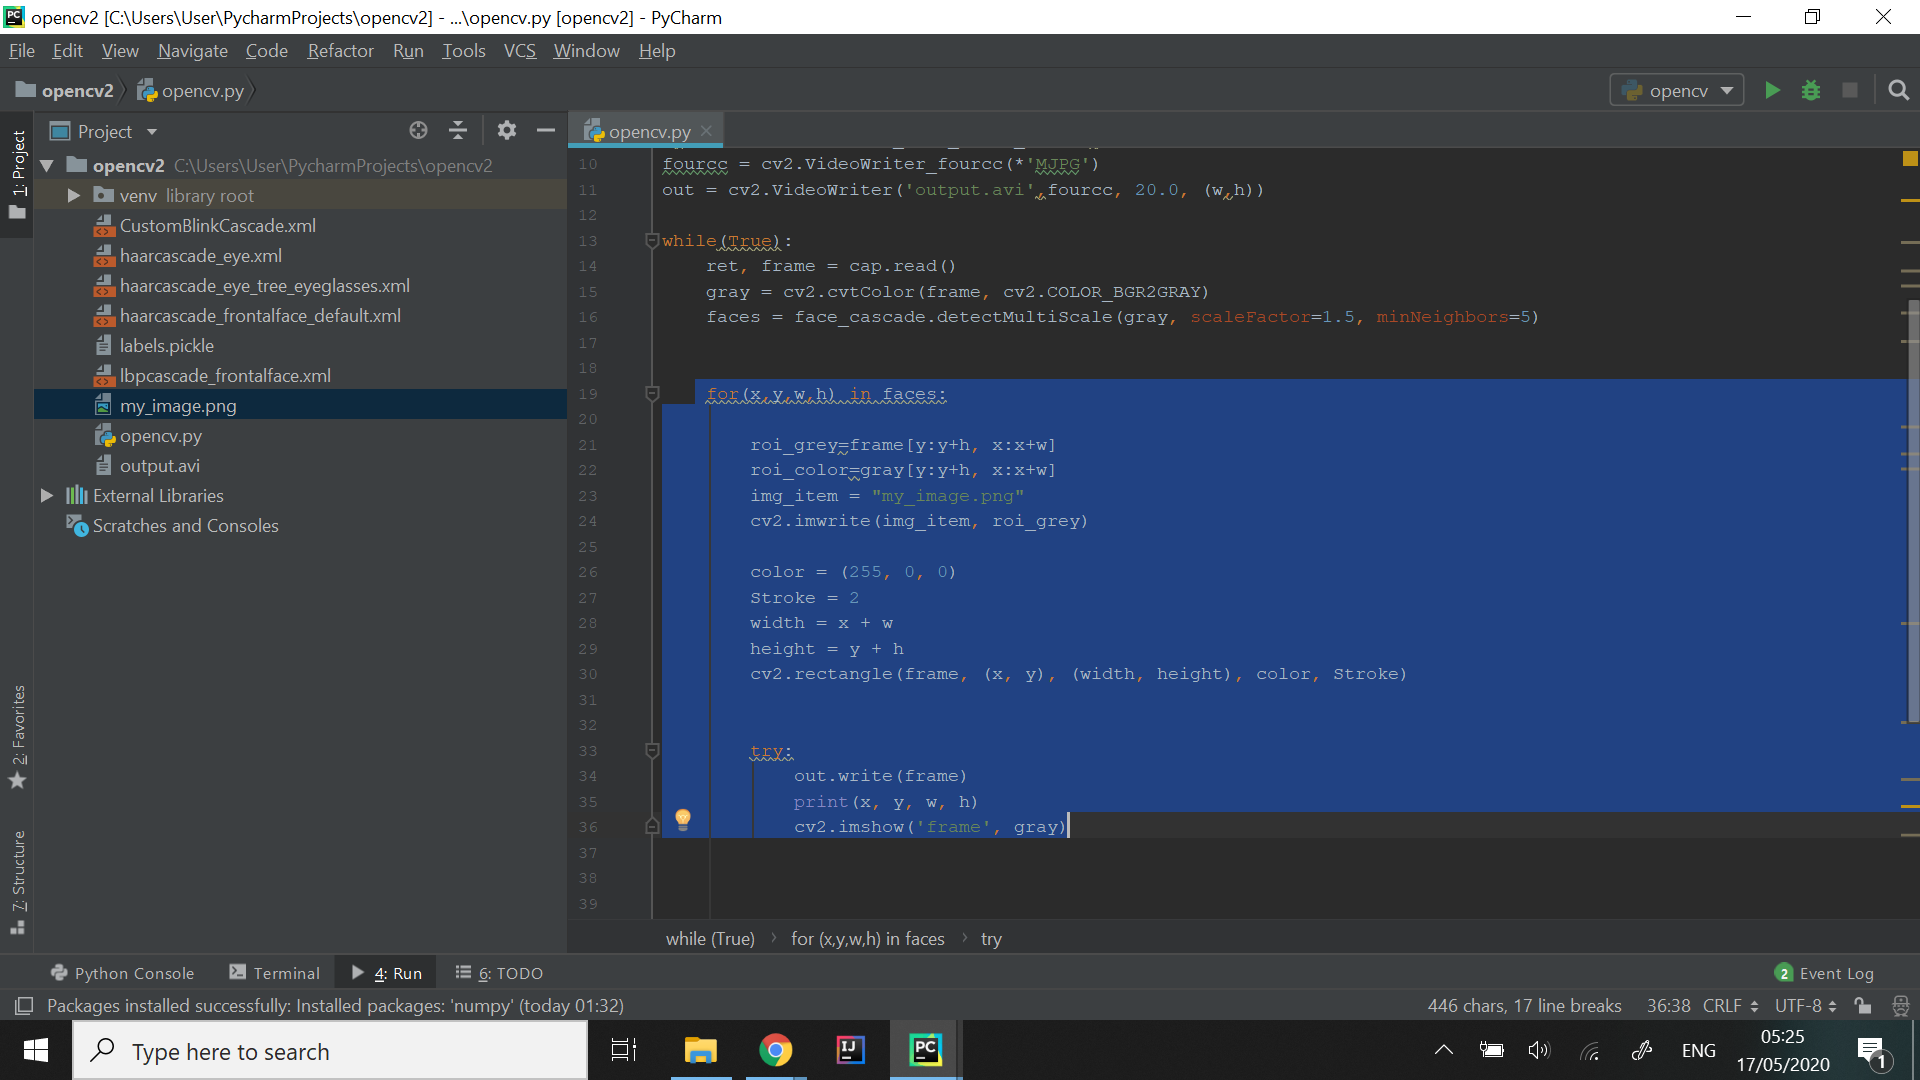
\includegraphics[width=0.8\textwidth]{Figures/facescript.png}
\end{figure}

\subsection{  Facial recognition and identification testing through video   }

when carrying out this test i made sure that i used my own image as a test for the system to identify myself and label me by my name when it has recognised me the system is performing the capture analysis of myself, I then will use other images to see if it can tell the difference between me and the random image. If my name pops up on the foreign individuals image that means the system has failed and the recognition isn't correct.

us\begin{figure}[h]
\includegraphics[width=0.8\textwidth]{Figures/facialidentification.png}
\end{figure}

As you can see by the above image the system has identified and recognised me, lets say we try another individual that as been trained by my system.


















\section{Results}
Summarise the output data, and the statistical or other techniques to deduce your results. Summarise your results, including tables or graphs as appropriate with a brief description of each. here possible, compare your results with other products/systems. Identify any possible threats to the validity of your results, and discuss each briefly here (you will discuss in more detail in the next chapter). % Conclusions and Term 2 work
\chapter{Discussion and Conclusions}
\label{chap:conclusions}
\lhead{\emph{Discussion and Conclusions}}
In this chapter, you should expand upon (and initially reflect upon) the discussion and conclusion of the research phase of the project. The expectation here is that you should discuss the results presented in the previous evaluation section of the project in their totality (i.e. as a whole) from which you will then draw clear conclusions both on the quantitative and qualitative aspects of the overall project. This chapter should be a about 2000 words long (5 pages of text - 1600 words of discussion and 400 words of conclusion). This may vary depending on quality. The conclusion section of this report should conclude the project.

Some suggested sections (the nature of this chapter should be discussed in detail with your term 2 supervisor):

\section{Solution Review}
Discuss how well your solution solves the problem, based on your results from the evaluation chapter.

\section{Project Review}
Discuss how well you addressed the project, and what you might do differently if you were to do it again. Make sure to identify how you handled any problems that arose during the project. Identify key skills that you learnt during the project, and clearly describe how you applied these, and how you might apply them differently if you were to do a similar project.[]

\section{Conclusion}
Enumerate the main conclusions you have got in terms of background, problem description and the solution approach you have come up with. Detail your primary and any secondary conclusions from your project.

\section{Future Work}
Discuss any proposals for completion of the project, or for enhancements, or for re-design of your solution or software. Enumerate all the things you would have wanted to do should you have more time to work on this project. % Conclusions and Term 2 work
\else
\chapter{Conclusions and Future Work}
\label{chap:conclusions}
\lhead{\emph{Conclusions}}
\section{Overview}
We now have some understanding of what a Drowsiness detection system is and this is very good,  as I enter into the implementation phase of my project things that I was confused about before I started my research have been clarified, certain areas I felt that I had a vague understanding of such things such as, how I will detect a persons face in a image. These self question marks have  have been clarified. Now I know that machine learning algorithms must be used and trained in order to achieve this task. 

\section{Discussion}
A major problem that I can reflect on during this Phase of the project was my time management, i honestly have to say that this must change and i must have a plan in place for the implementation phase of the project so that I can successfully achieve the requirements of my system without being stuck for time. Projects from other modules have played a major role in the delay of this being completed in a timely manner. If I used my time more wisely I feel that this project would have been completed with a greater quality and with much greater detail, however I must say I do feel accomplished as this is a very important piece of work and major work has gone into completing this research phase.

\section{Conclusion}
During the Background research I felt that this was the most essential piece of work that had to do as it clarified everything about the project that has been done in the past and present, also providing me with a very important understanding of how this project must be carried out. The background research portion helped me me learn large amounts of information about drowsiness detection systems and expand my knowledge on software solutions present that can aid with the implementation of my project.
During the problem definition portion of my project the main thing that I have taken away from completing this chapter is that I was able to pin point the exact problem that my project will be targeting when I'm implementing it in the future, This chapter helped my identify the best functional and non functional characteristics that my system must present in the final design. This chapter was the chapter that helped me identify new goals for my drowsiness detection system.
During my work on the  implementation approach I achieved many things, firstly i felt that this was the toughest chapter to complete as there were many questions I had to ask myself and a lot of decisions I had to make but the result of this was a very detailed mental visualisation of how I will develop my Project in the Implementation phase in semester 2, This chapter gave me different perspective on how I visualised my Project from how I will carry out my project to how I will mitigate the risks forcing me to develop a prototypes to that I can feel assured that the Technologies I have chosen are functional in my computer and thankfully they are.


\section{Future Work}

Overall I did achieve many things during this research phase but here have been many other things that I haven't achieved and wish I was able to accomplish. If I had more time allocated i would have added far more images and diagrams so that I can help explain and summarise a-lot of the explanations that I have provided through out this research phase, if i had more time I would have liked to added more to the Bibliography  in order to have a much fuller Background research and expand my knowledge even further on the Research undergone with Drowsiness detection, maybe if I had a bit more time i would have added more technologies and explored other technologies that i would have found interesting. Overall if i had more time i would have tried to build a prototype of a machine learning algorithm.





 % Conclusions and Term 2 work
\fi
%% ----------------------------------------------------------------
\label{Bibliography}
\bibliographystyle{IEEEtranN}  % Use the "IEEE Transaction" BibTeX style for formatting the Bibliography
\bibliography{Bibliography}  % The references (bibliography) information are stored in the file named "Bibliography.bib"
\lhead{\emph{Bibliography}}  % Change the left side page header to "Bibliography"

%% ----------------------------------------------------------------
% Now begin the Appendices, including them as separate files

\addtocontents{toc}{\vspace{2em}} % Add a gap in the Contents, for aesthetics

\appendix % Cue to tell LaTeX that the following 'chapters' are Appendices

\chapter{Code Snippets}

Put appendix material in this section e.g. code snippets 

USE THE APPENDICES	% Appendix Title

\chapter{Wireframe Models} % Appendix Title

%\input{Appendices/AppendixC} % Appendix Title

\addtocontents{toc}{\vspace{2em}}  % Add a gap in the Contents, for aesthetics
\backmatter
\end{document}  % The End
%% ----------------------------------------------------------------